\chapter{Material and Methods}\label{chap:material_and_methods}

\section{Toxicity Data and Processing}\label{sec:invitrodb}
\subsection{ToxCast invitroDB v4.1}
The most recent release of the ToxCast's database, referred to as \emph{invitroDBv4.1}, serves as a source of an extensive collection of HTS targeted bioactivity data (~100 GB). This database encompasses information on a total of $\num{10196}$ compounds, selectively tested across 1485 assay endpoints.
Assay endpoints themselves stem from assays, please refer Figure~\ref{fig:toxcast_db_annotations_recolored} for an overview of the assay annotaion structure.

\begin{figure}  % Placement options: h (here), t (top), b (bottom), p (page)
    \centering
    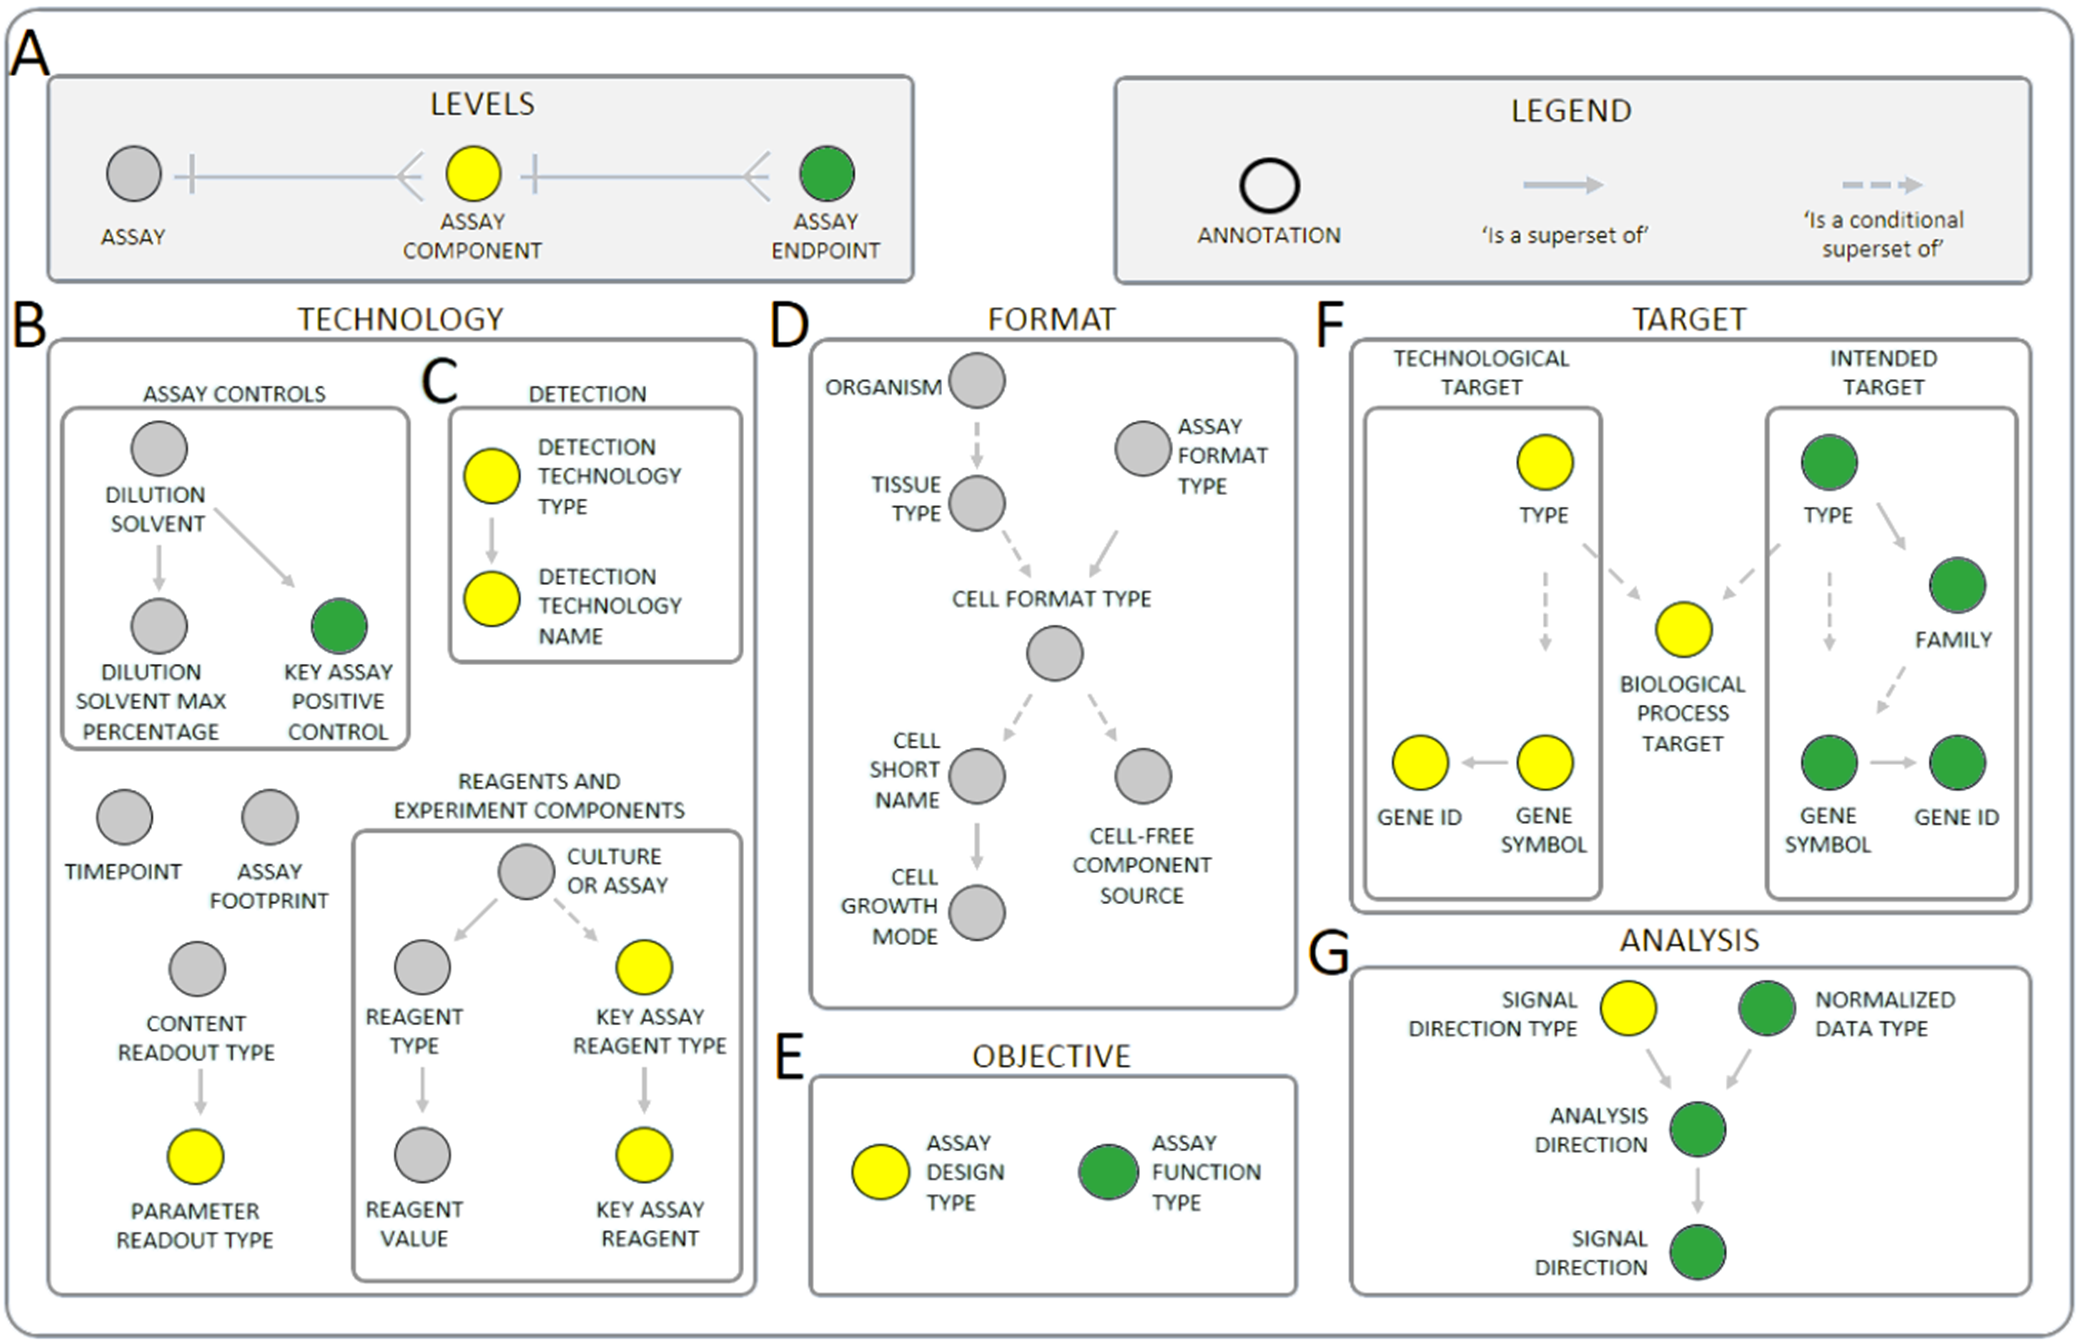
\includegraphics[width=1.0\textwidth]{figures/toxcast_db_annotations_recolored.png}  
    \caption{Assay endpoints are annotated with (A) assay
    identification information, (B) design information, (C) target information, and (D) analysis information. Relationships between annotations are either one-to-many or conditional where certain dependencies may not be applicable. Adapted Figure obtained from~\cite{userguide}.}
~\label{fig:toxcast_db_annotations_recolored} 
\end{figure}

The assays utilize a range of technologies to assess the impact of chemical compounds on a wide array of biological targets, including individual proteins and cellular processes such as mitochondrial health, developmental processes and nuclear receptor signaling. This resource originates from the collaboration of two prominent institutions: the  U.S. EPA through its ToxCast program and the National Institutes of Health (NIH) via the Tox21 initiative. Using data collected from multiple research labs (refer to Table~\ref{tab:laboratories} in the Appendix), this relational database is accessible to the public and can be downloaded\footnote{\url{https://www.epa.gov/chemical-research/exploring-toxcast-data}, released on Sept 21, 2023} by visiting the official ToxCast website.

\subsection{tcpl v3.0}
The \emph{tcpl}\footnote{\url{https://github.com/USEPA/CompTox-ToxCast-tcpl}} package provides a wide range of tools for efficiently managing HTS data. It enables reproducible concentration-response modeling and populates the \texttt{MYSQL} database, invitroDBv4.1. The multiple-concentration screening paradigm intends to pinpoint the bioactivity of compounds, while also estimating their efficacy and potency. 

In Section~\ref{sec:pytcpl}, we introduce \emph{pytcpl} a \texttt{Python} reimplementation of the vital components that underpin the entire ToxCast pipeline. It should be noted that these components, as presented in the following, are applicable to both tcpl and pytcpl.

\subsection{Efficacy Cutoff}
The \emph{efficacy cutoff}, unique to each assay endpoint and illustrated for a single tested compound in Figure~\ref{fig:concentration_response_series}, plays a significant role in evaluating the compound's bioactivity. It serves as a threshold that differentiates active and inactive compounds, essentially defining the minimum response level that is biologically relevant. The process of establishing this threshold involves estimating the noise level in the assay responses.

\subsection{Concentration-Response Series}
Each compound $c_j$ tested within an assay endpoint $a_i$ involves the collection of the respective \emph{concentration-response series (CRS)} denoted as $CRS_{ij}$, showcased in Figure~\ref{fig:concentration_response_series}. A CRS is represented as a set of concentration-response pairs: 
\[ CRS_{i,j} = \{(conc_{1_{i,j}}, resp_{1_{i,j}}), (conc_{2_{i,j}}, resp_{2_{i,j}}), \dots, (conc_{n_{\text{datapoints}_{i,j}}}, resp_{n_{\text{datapoints}_{i,j}}})\} \] where $n_{\text{datapoints}_{i,j}}$ varies based on the number of concentrations tested. 

\begin{figure}
    \centering
    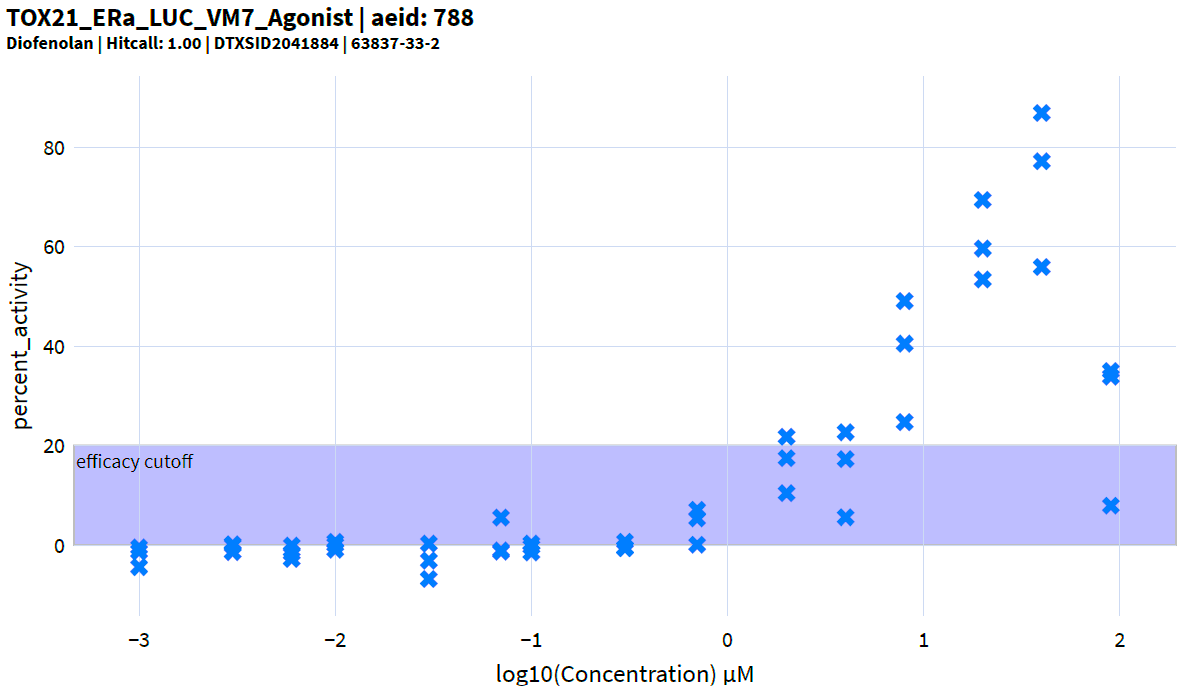
\includegraphics[width=1.0\textwidth]{figures/CRS.png}  
    \caption{The CRS belongs to \emph{Diofenolan} (DTXSID2041884), tested in the assay endpoint \emph{TOX21\_ERa\_LUC\_VM7\_Agonist} (aeid=788). The shaded region represents the estimated efficacy cutoff. This particular series comprises a total of $k = 45$ concentration-response pairs and is structured into $n_{conc} = 15$ distinct concentration groups, with each group consisting of $n_{rep} = 3$ replicates. }
~\label{fig:concentration_response_series} 
\end{figure}

In practice, concentrations are often subjected to multiple testing iterations, resulting in the distinct concentration groups with replicates. Table~\ref{tab:concentrations_quantities} presents the key quantities associated with an individual CRS when considering a specific assay endpoint $a_i$ and compound $c_i$. To visualize the variations in these metrics across the complete set of analyzed CRS in this work, please refer to Figure~\ref{fig:concentration_metric_distributions} in the Appendix. 

\begin{table}
    \centering
    \caption{Description of Parameters}
    \label{tab:concentrations_quantities}
    \begin{tabular}{ll}
        \toprule
        \textbf{Quantity} & \textbf{Description} \\
        \midrule
        $n_{\text{datapoints}_{i,j}}$ & Total number of concentration-response pairs ($|CRS|$) \\
        $n_{\text{groups}_{i,j}}$ & Number of distinct concentrations tested \\
        $n_{\text{replicates}_{i,j}}$ & Number of replicates for each concentration group \\
        $min_{\text{conc}_{i,j}}$ & Lowest concentration tested \\
        $max_{\text{conc}_{i,j}}$ & Highest concentration tested \\
        \bottomrule
    \end{tabular}
\end{table}

Concentration-response pairs, along with essential sample information such as well type and assay well-plate indices, can be retrieved by combining tables \emph{mc0}, \emph{mc1}, and \emph{mc3} from invitroDBv4.1, which represent the raw data. A special role is assigned to the control wells, which typically contain untreated samples or samples with a known, non-toxic response. They are used as a baseline to normalize the treated samples and account for any background noise in the assay~\cite{sheffield2021}. The concentrations are transformed to the logarithmic scale in micromolar, while the responses are control well-normalized to either fold-induction or percent-of-control activity:

\begin{enumerate}
    \item \textbf{Fold Induction}: is a measure used to quantify how much, for instance, gene expression has changed in response to a treatment compared to its baseline level from the control well set. E.g., if a gene is expressed five times higher in a treated sample compared to the control, the fold induction would be 5.
    \item \textbf{Percent of Control}: is another way to express the relative change in a activity due to a treatment compared to the control.
\end{enumerate}


\subsection{tcplFit2}\label{sec:tcplfit2}
\emph{TcplFit2}\footnote{\url{https://github.com/USEPA/CompTox-ToxCast-tcplFit2}} is an extension to tcpl, focused on curve-fitting and hit-calling. The package also offers a flexible and robust fitting procedure, allowing for the use of different optimization algorithms and the incorporation of user-defined constraints. This sets it apart from other open-source CSS modeling packages such as \emph{drc} and \emph{mixtox}, as it is explicitly designed for HTS concentration-response data.

\subsection{Curve Fitting}
All the curve fit models from tcplFit2, as outlined in Table~\ref{tab:tcplfit2_models} and showcased in Figure~\ref{fig:tcplfit2_models}, assume that the normalized observations in the CRS conform to a Student's $t$-distribution with 4 degrees of freedom~\cite{tcplv3.0}. The Student's $t$-distribution has heavier tails compared to the normal distribution, making it more robust to outlier and eliminates the necessity of removing potential outliers prior to the fitting process. The model fitting algorithm in tcplFit2 employs nonlinear \emph{maximum likelihood estimation (MLE)} to determine the model parameters for all available models.
% \afterpage{
%     \clearpage % Insert a page break before the table and figure
\begin{table}
    \centering
    \begin{threeparttable}[b]
    \caption{tcplfit2 Model Details}
    \renewcommand{\arraystretch}{1.1}
    \begin{tabular}{lll}
    \toprule
    \textbf{Model} & \textbf{Label} & \textbf{Equations\tnote{1}} \\
    \midrule
    Constant & constant & \(f(x) = 0\) \\ 
    Linear & poly1 & \(f(x) = ax\) \\ 
    Quadratic & poly2 & \(f(x) = a\left(\frac{x}{b} + {\left(\frac{x}{b}\right)}^{2}\right)\) \\ 
    Power & power & \(f(x) = ax^p\) \\ 
    Hill & hill & \(f(x) = \frac{tp}{1 + {\left(\frac{ga}{x}\right)}^{p}}\) \\ 
    Gain-Loss & gnls & \(f(x) = \frac{tp}{(1 + {\left(\frac{ga}{x}\right)}^{p})(1 + {\left(\frac{x}{la}\right)}^{q})}\) \\ 
    Exponential 2 & exp2 & \(f(x) = a\left(\exp\left(\frac{x}{b}\right) - 1\right)\) \\
    Exponential 3 & exp3 & \(f(x) = a\left(\exp\left({\left(\frac{x}{b}\right)}^{p}\right) - 1\right)\) \\
    Exponential 4 & exp4 & \(f(x) = tp\left(1 - 2^{-\frac{x}{ga}}\right)\) \\
    Exponential 5 & exp5 & \(f(x) = tp{\left(1 - 2^{-(\frac{x}{ga})^{p}}\right)}\) \\
    \bottomrule
    \end{tabular}
    \begin{tablenotes}
        \item [1] Parameters: $a$: x-scale, $b$: y-scale $p$: (gain) power, $q$: (loss) power, $tp$: top, $ga$: gain AC50, $la$: loss AC50
    \end{tablenotes}
~\label{tab:tcplfit2_models}
\end{threeparttable}
\end{table}

\begin{figure}  % Placement options: h (here), t (top), b (bottom), p (page)
    \centering
    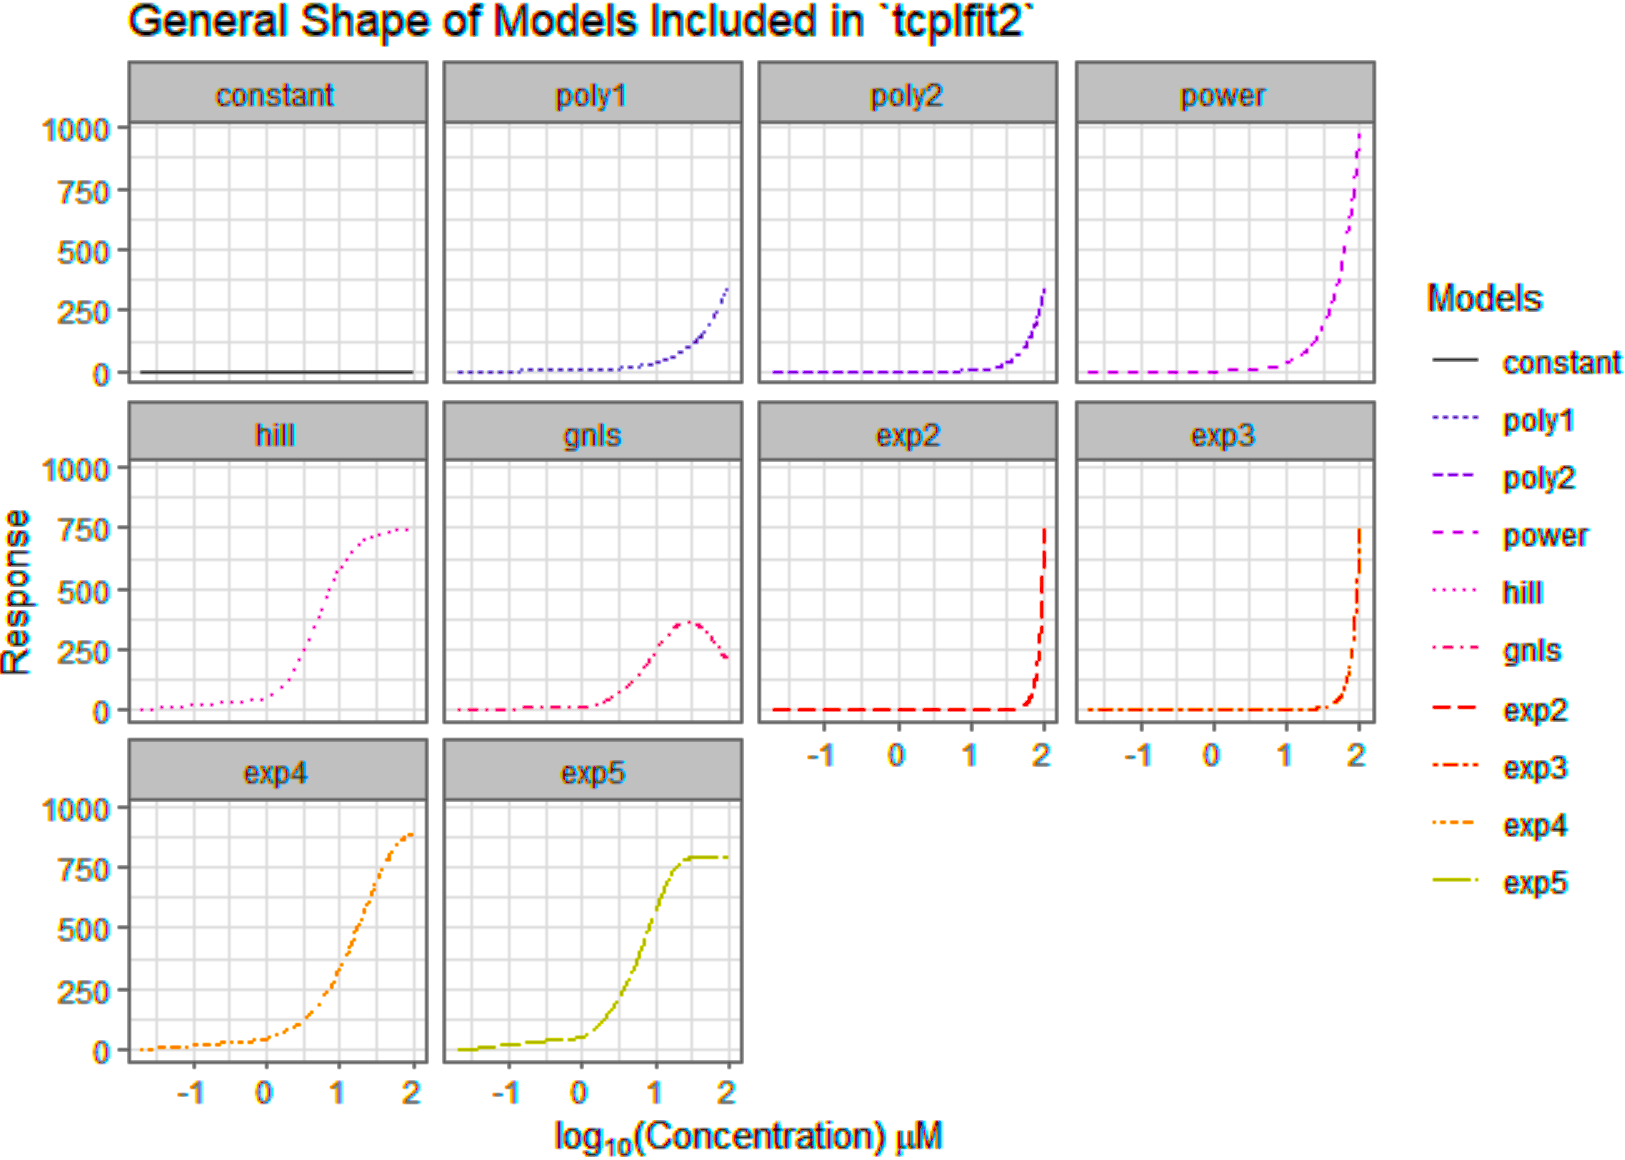
\includegraphics[width=0.9\textwidth]{figures/fit_models.png}
    \caption{Employed curve-fit models in tcpl v3.0 for fitting concentration-response data series through the application of maximum likelihood estimation. Figure obtained from~\cite{tcplv3.0}.}
~\label{fig:tcplfit2_models}
\end{figure}

% \clearpage % Insert another page break after the table and figure
% }

Consider $t(z, \nu)$ as the Student's $t$-distribution with $\nu$ degrees of freedom, where $y_i$ represents the observed response for the $i$-th observation, and $\mu_i$ is the estimated response for the same observation. The calculation of $z_i$ is as follows: $z_i = y_i - \mu_i \exp(\sigma)$, where $\sigma$ is the scale term. Then the log-likelihood is: $\sum_{i=1}^n [\ln(t(z_i,4)) - \sigma]$, where $n$ is the number of observations.

The \emph{Akaike Information Criterion (AIC)} is used as measure of goodness of fit, defined by the formula: $AIC = -2\log(L(\hat{\theta}, y)) + 2K$, where $L(\hat{\theta}, y)$ is the likelihood of the model given the data and $K$ is the number of model parameters. The model with the lowest AIC value is chosen as the \emph{winning} model. The winning model is then used to estimate the efficacy and potency of the compound. The potency estimates, also called \emph{point-of-departure (POD)} estimates, are derived from the fitted curve, identifying certain \emph{activity concentrations (AC)} at which the curve first reaches certain response levels. Central POD estimates are depicted graphically in Figure~\ref{fig:active_and_pod}.

\begin{figure}[htbp]
    \centering
    \begin{subfigure}[b]{0.48\textwidth}
        \centering
        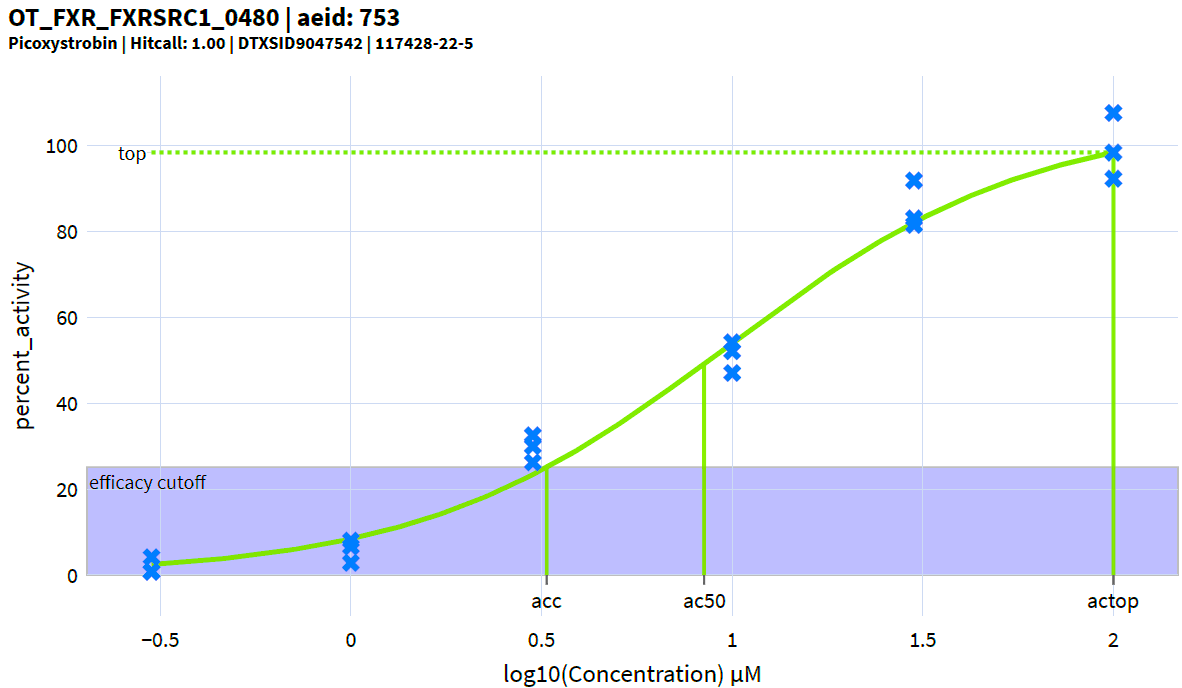
\includegraphics[width=\textwidth]{figures/POD.png}
        \caption{POD estimates for the chemical \emph{Picoxystrobin} (DTXSID9047542) tested in the assay endpoint with $aeid=753$. The efficacy cutoff is defined at 25 percent-of-control activity. The winning fit model was the Hill function.~\emph{ACC}: The AC at the efficacy cutoff is at $3.3 \mu M$.~\emph{AC50}: The AC at $50\%$ of the maximum response is at $8.4 \mu M$.~\emph{ACtop}: The AC at the maximum response is at $100 \mu M$.}
    ~\label{fig:active_and_pod}
    \end{subfigure}
    \hfill
    \begin{subfigure}[b]{0.48\textwidth}
        \centering
        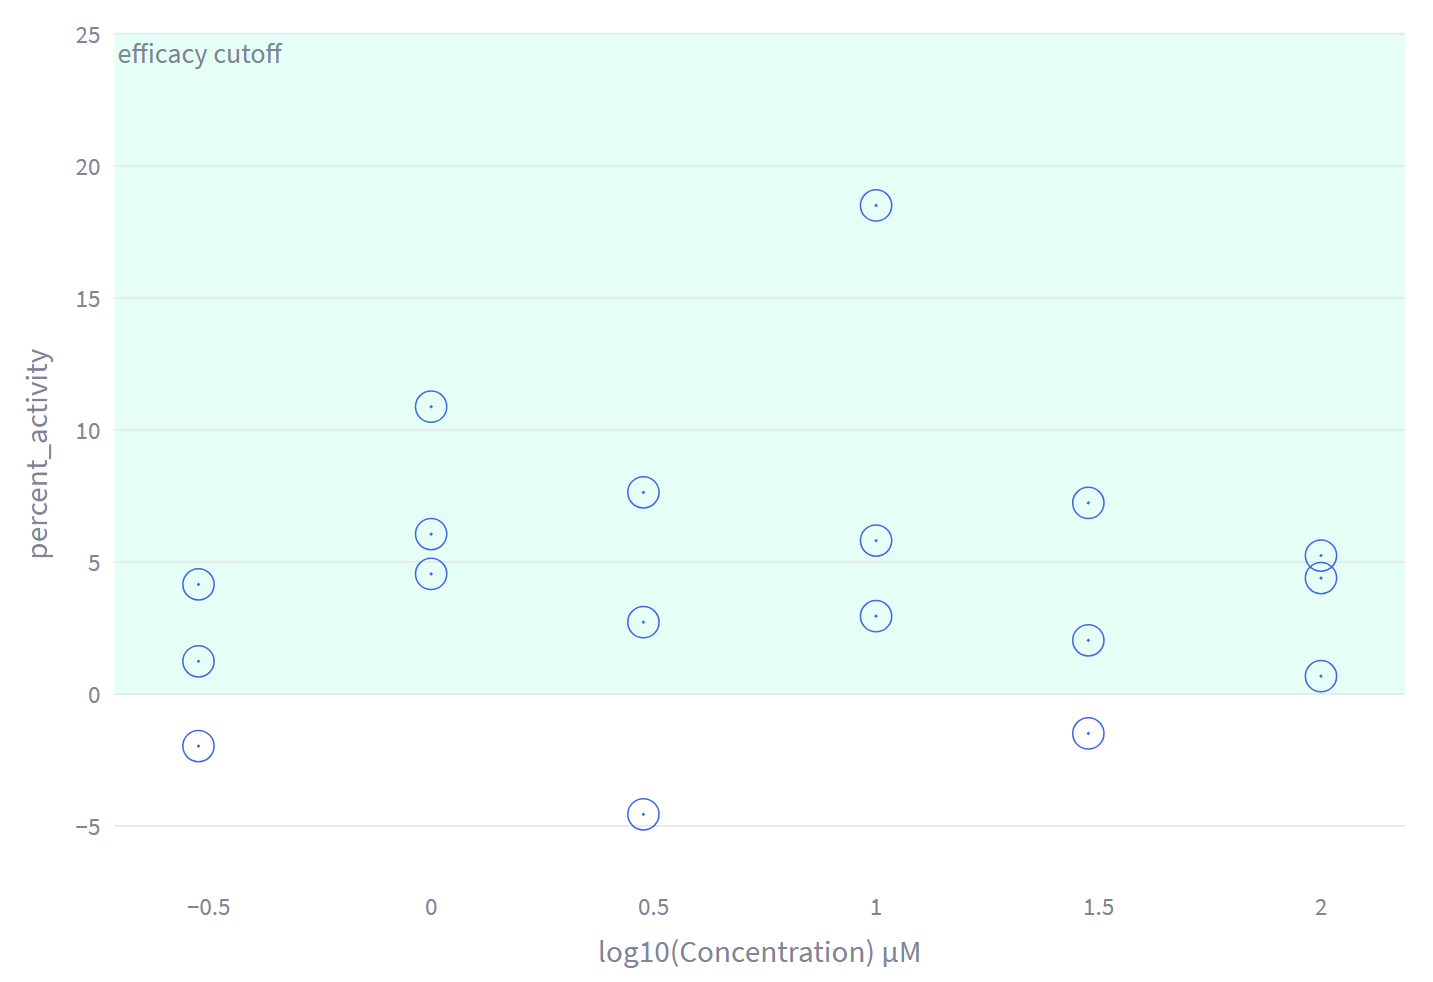
\includegraphics[width=\textwidth]{figures/inactive_and_no_pod.png}
        \caption{POD estimates are not available for the chemical compound \emph{PharmaGSID\_48518} (DTXSID9048518) tested in the same assay endpoint as shown in the left figure. In this case, was unnecessary as no response reached or exceeded $80\%$ of the efficacy cutoff, clearly indicating the inactivity of the compound. In such scenarios, a calculation of POD estimates is not applicable.}
        ~\label{fig:inactive_and_no_pod}
    \end{subfigure}
    \caption{Presence Matrix: assay endpoint-compound relationship.}
    ~\label{fig:pod}
\end{figure}


\subsection{Hit Calling}
The \emph{continuous hitcall} is a measure of the probability that a compound is active, calculated based on the product of the following three probability values~\cite{sheffield2021}:

\begin{enumerate}[i.]
    \item that at least one median response is greater than the efficacy cutoff, computed by using the error parameter from the model fit and Student $t$-distribution to calculate the odds of at least one response exceeding the efficacy cutoff;
    \item that the top of the winning fitted curve is above the cutoff which is the likelihood ratio of the one-sided probability of the efficacy cutoff being exceeded;
    \item that the winning AIC value is less than that of the constant model:
    \begin{equation}
    \frac{e^{-\frac{1}{2}AIC_{\text{winning}}}}{e^{-\frac{1}{2}AIC_{\text{winning}}} + e^{-\frac{1}{2}AIC_{\text{cnst}}} }
    \end{equation}
\end{enumerate}

In certain instances, compounds underwent multiple tests within a single assay endpoint, leading to their association with multiple CRS. In these exceptional cases, a hitcall is computed for each CRS, and then highest hitcall value is recorded as the compound's ultimate hitcall.

\subsection{Flagging}
Finally, after processing, each CRS is assigned to an appropriate fit category based on the level of certainty in the estimated bioactivity. Additionally, cautionary flags are assigned to account for problematic data series or or uncertainties related fits and hits.


\section{New Toxicity Pipeline Implementation: pytcpl}\label{sec:pytcpl}
\subsection{Introduction} 
This thesis introduces \emph{pytcpl}\footnote{\url{https://github.com/rbBosshard/pytcpl}}, a streamlined \texttt{Python} repository inspired by the \texttt{R} packages \emph{tcpl} and {tcplfit2}. The package optimizes data storage and generates compressed \texttt{Parquet} files of the relevant raw data and metadata from \emph{invitroDBv4.1}. Exclusively utilizing this repository eliminates the need for a complex and extensive database installation, rendering downstream analysis more accessible and efficient. Our package is crafted to accomodate cusomizable processing steps and facilitate interactive data visualization with an own \emph{Curve Surfer}\footnote{\url{https://pytcpl.streamlit.app/}}. Furthermore, it enables researchers who prefer \texttt{Python} to easily participate in data analysis and exploration, overcoming any limitations associated with using \texttt{R} code.

The pytcpl pipeline adds an additional setup and post-processing step around the main pipeline:
\begin{itemize}
    \item \textbf{Setup}: This step involves user-specified subsetting of assay endpoints, tagging assays with external assay annotations, enabling workload balancing for distributed processing and generating \texttt{Parquet} files from all raw and metadata, optionally for database decoupled analysis.
    \item \textbf{Main} (similar to tcpl+tcplFit2): This step involves cutoff determination, curve fitting, hit calling and flagging.
    \item \textbf{Post-Processing}: This step has the goal of improving the overall quality of the data and involves post-processing curation, cytotoxicity interference reevaluation and the custom export of the final results.
\end{itemize}

\subsection{Setup step}\label{sec:subset_data}
\subsubsection{Subsetting Data}
For a better data comprehension, the presence matrix denoted as $P \in {{0, 1}}^{m \times n}$ is introduced. In this matrix, rows (indexed by $i$) represent assay endpoints $a_i$, and columns (indexed by $j$) indicate whether testing was performed (1) or not performed (0) for compound $c_j$ in those endpoints. Due to selective compound testing across different assay endpoints, matrix $P$ is sparse. For a visual representation of the presence matrix $P$ covering all assay endpoints and compounds in \textit{invitroDBv4.1}, refer to Figure~\ref{fig:presence_matrix_all}.

\begin{figure}[htbp]
    \centering
    \begin{subfigure}[b]{0.48\textwidth}
        \centering
        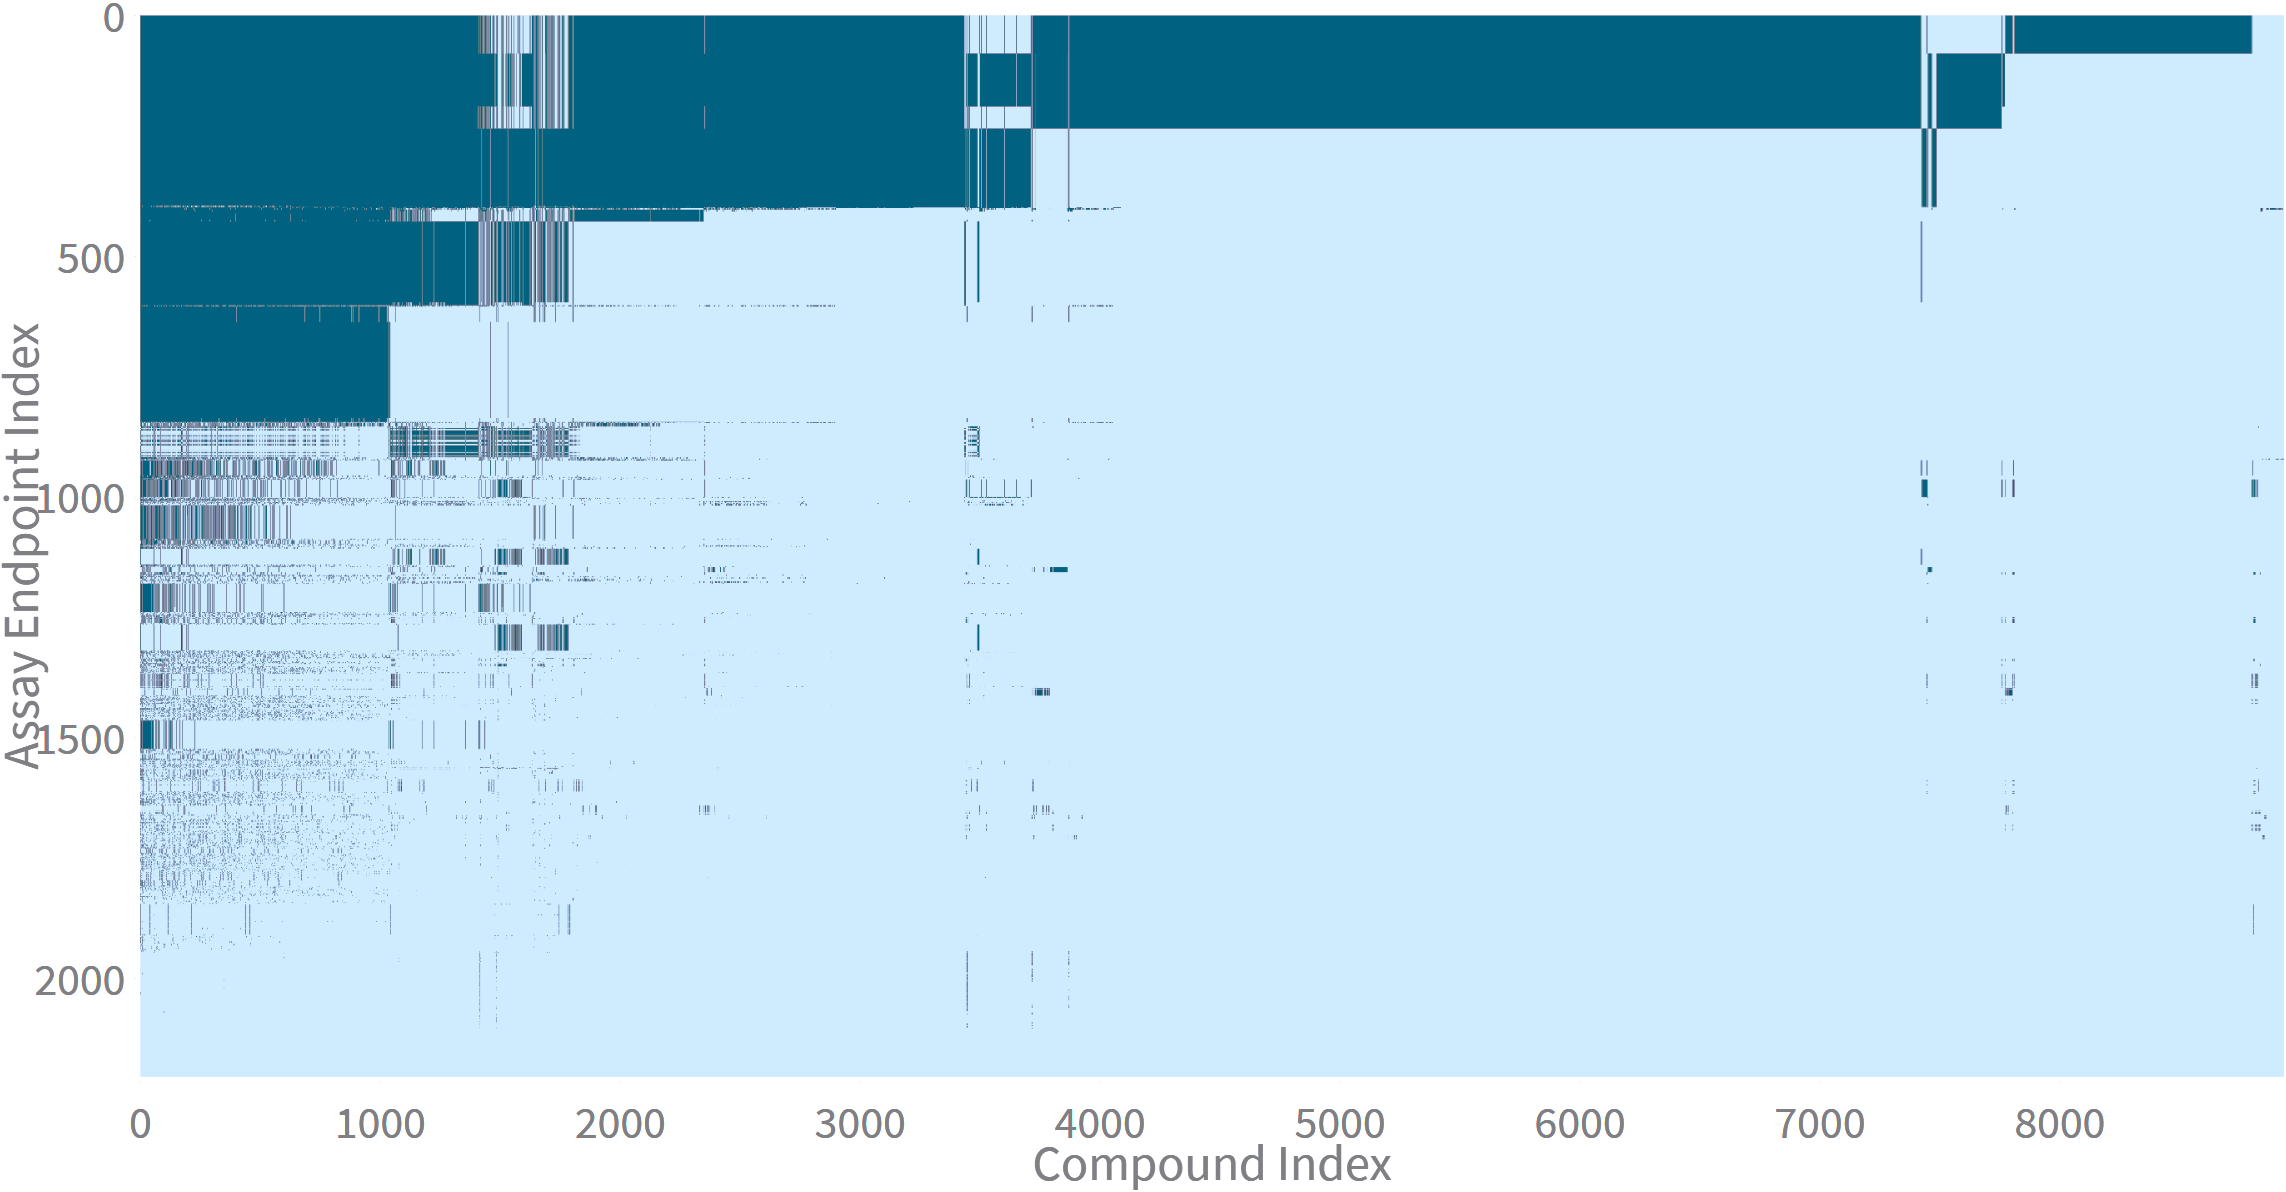
\includegraphics[width=\textwidth]{figures/presence_matrix_all.png}
        \caption{The presence matrix $P_{\text{all}}$, covers all assay endpoints and compounds from \emph{invitroDBv4.1}, totaling $m = \num{2205}$ assay endpoints and $n = \num{8935}$ compounds, excluding 606 compounds lacking molecular fingerprints. When $P_{\text{all}_{ij}} = 1$, there are \num{3196178} CRS available for analysis}
    ~\label{fig:presence_matrix_all}
    \end{subfigure}
    \hfill
    \begin{subfigure}[b]{0.48\textwidth}
        \centering
        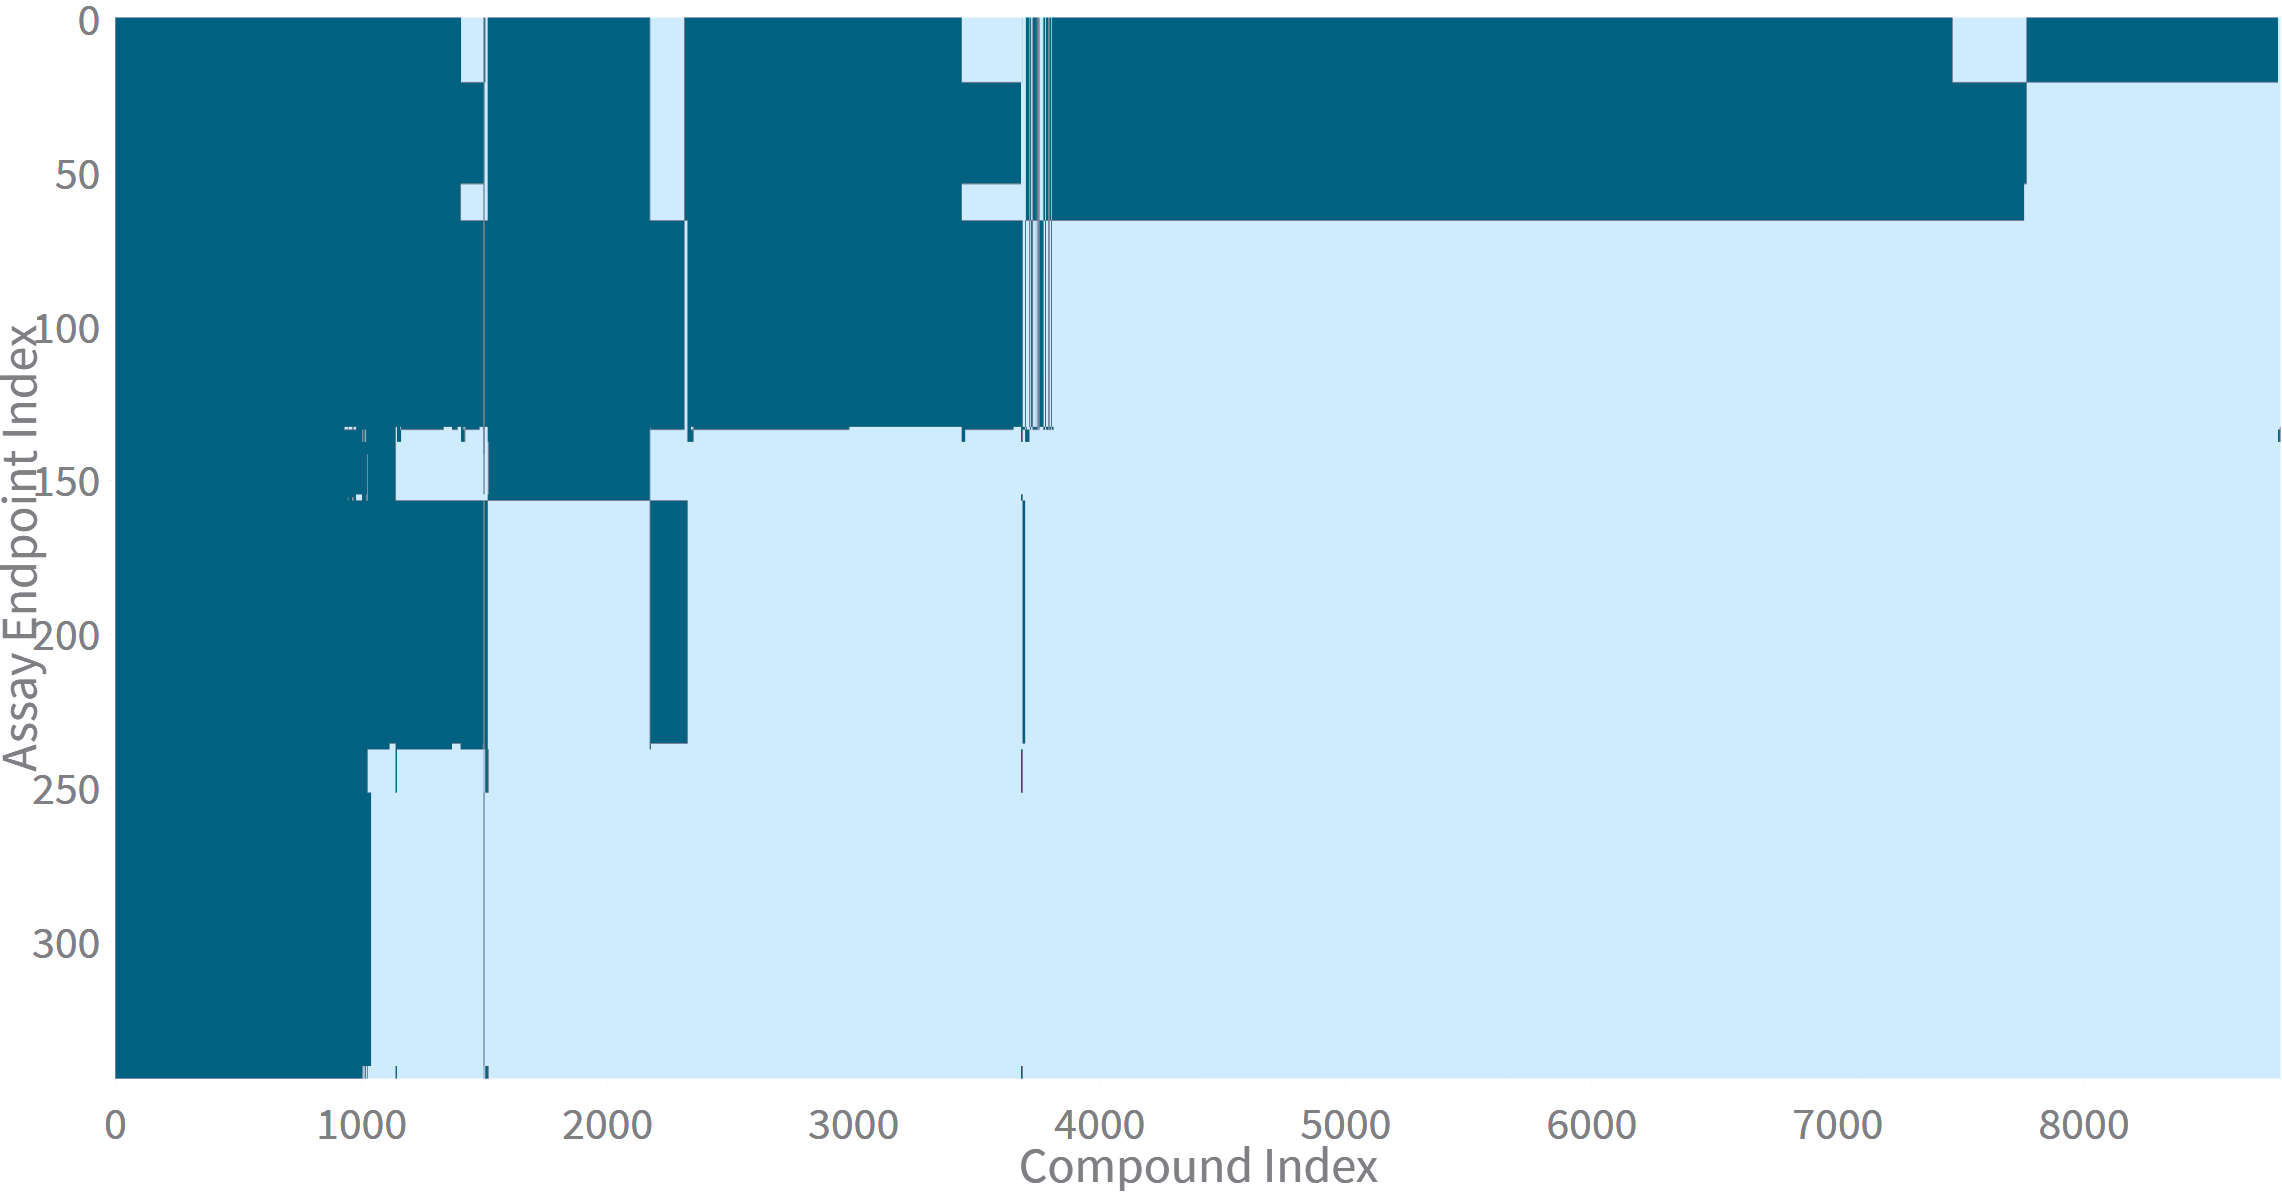
\includegraphics[width=\textwidth]{figures/presence_matrix_subset.png}
        \caption{$P_{subset}$ covers a specific subset of relevant assay endpoints and compounds considered for this thesis, totaling $m = \num{345}$ assay endpoints and $n = \num{8804}$ compounds. Assayy endpoints with less then 1000 tested compounds were omitted. When $P_{\text{subset}_{ij}} = 1$, there are \num{1043222} CRS available for analysis.}
        ~\label{fig:presence_matrix_subset}
    \end{subfigure}
    \caption{Presence Matrix: In both (a) and (b), structured by ranking according to the number of compounds associated with each assay endpoint, with compounds sorted in descending order
    of their occurrence frequency.}
    ~\label{fig:presence_matrix}
\end{figure}

In this thesis, we exclusively considered assay endpoints that had been tested with a minimum of $\num{1000}$ compounds. This selection criterion ensures the presence of adequate data for subsequent training of robust machine learning models. You can refer to Figure~\ref{fig:presence_matrix_subset} for a visual representation of the presence matrix $P$ which includes only this particular subset of assay endpoints. From this moment forward, we will refer to this specific subset as the \emph{dataset}, which will be the focus of this thesis. 

\subsubsection{Exernal Assay Annotation}
The assay endpoints were tagged with external annotations that involve, the attributed toxcity endpoint, the type of mechanistic target and the Mode of Action.

The investigated assay endpoints are enriched with external annotations attributed by the Integrated Chemical Environment (ICE)~\cite{ice2022}, which provide valuable context and information about each endpoint. These annotations encompass the following aspects:

\begin{enumerate}
    \item \textbf{Toxicity Endpoint}: This annotation specifies the type of toxicity or adverse effect associated with each assay endpoint, helping to clarify the specific aspect of toxicity under investigation.
    
    \item \textbf{Mechanistic Target}: This annotation sheds light on the particular target mechanism or biological pathway being studied.
    
    \item \textbf{Mode of Action}: The annotations also describe how the tested compounds interact with the mechanistic targets andprovides insights into the underlying biological processes or actions involved.
\end{enumerate}

\subsection{Main step}
The pytcpl main pipeline is similar to the \texttt{R}-based tcpl+tcplFit2 pipeline, with the exception of the curve fitting stage where the pytcpl pipeline made a notable modification by excluding a suboptimal model and including a novel model. The removal of Exponential 3 model was due to its suboptimal capability in fitting models within the original tcpl pipeline. Furthermore, an additional Gain-Loss 2 model was introduced during the curve-fitting stage. This secondary model has one fewer model parameter than the primary Gain-Loss 1 model, which helps mitigate the risk of overfitting CRS data. Table~\ref{table:pytcpl_models} provides an overview of these changes within the pytcpl pipeline for reference.

\begin{table}
    \caption{pytcpl Model Updates}~\label{table:pytcpl_models}
    \centering
    \begin{threeparttable}[b]
    \renewcommand{\arraystretch}{1.4}
    \begin{tabular}{lccc}
    \toprule
    \textbf{Model} & \textbf{Label} & \textbf{Equations\tnote{1}} & \textbf{Role in pytcpl} \\
    \midrule
    Exponential 3 & exp3 & \(f(x) = a\left(\exp\left({\left(\frac{x}{b}\right)}^{p}\right) - 1\right)\) & Omitted \\
    Gain-Loss 2 & gnls2 & \(f(x) = \frac{tp}{1 + {\left(\frac{ga}{x}\right)}^{p}}\exp\left({-qx}\right)\) & New \\
    \bottomrule
    \end{tabular}
    \begin{tablenotes}
        \item [1] Parameters: $a$: x-scale, $b$: y-scale $p$: (gain) power, $q$: (loss) power, $tp$: top, $ga$: gain AC50
    \end{tablenotes}
\end{threeparttable}
\end{table}

\subsection{Post-Processing step}
\subsubsection{Post-Processing Curation}
Following the ICE guidelines\footnote{\url{https://ice.ntp.niehs.nih.gov/DATASETDESCRIPTION?section=cHTS}}, quality filters were implemented to enhance the processed concentration-response series. This step introduces OMIT/PASS curation warning flags, which could be applied either based on assay endpoints or compound quality control criteria.

\subsubsection{Cytotoxicity Interference Reevaluation}
As previously discussed in Chapter~\ref{chap:background}, the assessment of compound toxicity can be complicated by the presence of non-specific cytotoxic responses. In this section, we delve into the exploration of a method for reevaluating the reported hitcall status of active compounds, considering the estimated extent of cytotoxicity interference. The cytotoxicity of a compound in a target assay endpoint may be assessed by comparing the activity concentration at the efficacy cutoff, represented as $ACC_{\text{target}}$, with that of its corresponding viability assay endpoint counterpart (as shown in Figure~\ref{fig:aeid_acid_aid}), referred to as $ACC_{\text{cyto}}$. 

\begin{figure} 
    \centering
    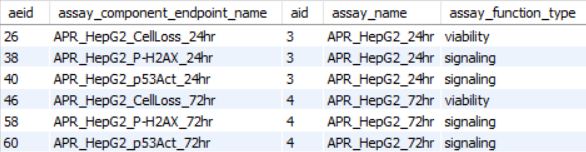
\includegraphics[width=0.8\textwidth]{figures/aeid_acid_aid.png}
    \caption{Each assay endpoint has an assay identifier (aid) used to match it with its viability counterpart that assesses cell loss. In this example, \emph{APR\_HepG2\_CellLoss\_24hr} (aeid=26) corresponds to aeid=38 and aeid=40. Similarly, \emph{APR\_HepG2\_CellLoss\_72hr} (aeid=46) corresponds to aeid=58 and aeid=60.}
~\label{fig:aeid_acid_aid}
\end{figure}

If no counterpart is available in the database, we presented in the following a statistical approach that allows for a cytotoxicity estimate. It uses the median ACC for the compound of interest across a set of assay endpoints dedicted for capturing the cytotoxicity burst. 
The ACC is assumed to have a Gaussian error distribution. Cytotoxicity in terms of the respective potencies is assumed when: $ACC_{\text{cyto}} \leq ACC_{\text{target}}$. The probability can be expressed as:

\[
P(\text{cytotoxic}) = P(ACC_{\text{cyto}} - ACC_{\text{target}} \leq 0) = \Phi\left(\frac{ACC_{\text{cyto}} - ACC_{\text{target}}}{\sqrt{\text{SD}_{ACC_{\text{cyto}}}^2 + \text{SD}_{ACC_{\text{target}}}^2 }}\right)
\]
    
where $\Phi$ is the Gaussian cumulative distribution function. The standard deviations $\text{SD}_{ACC_{\text{cyto}}}$ and $\text{SD}_{ACC_{\text{target}}}$ are unknown but are estimated as $0.3 \log_{10}$ ${\mu M}$ units~\cite{watt2018}. 

For the statistical approach with the burst assays, $\text{SD}_{ACC_{\text{cyto}}}$ can be derived from the median absolute deviation (MAD) of the respective ACC values. Additionally, $P(\text{cytotoxic})$ is muliplied by $\frac{n_{\text{hit}}}{n_{\text{tested}}}$, the ratio of the number where the compound was considerd active divided by the number of cytotoxicity burst assay endpoints where the compound was tested. 

Ultitmately, $P(\text{cytotoxic})$ is then mulitplied with the original continuous hitcall of active compounds. The final cytotoxicity-corrected hitcall is then defined as follows: $\text{hitcall}_{\text{c}} = \text{hitcall}_{\text{original}} * (1 - P(\text{cytotoxic}))$.

\subsection{Curve Surfer}
Figure~\ref{fig:curve_surfer} presents the developed \emph{Curve Surfer}, a browser-based application that enables interactive data exploration and visualization of the processed data. The curve surfer tool is built using Streamlit, an open-source Python library that makes it easy to build custom web-apps for machine learning and data science. 

\begin{figure}  % Placement options: h (here), t (top), b (bottom), p (page)
    \centering
    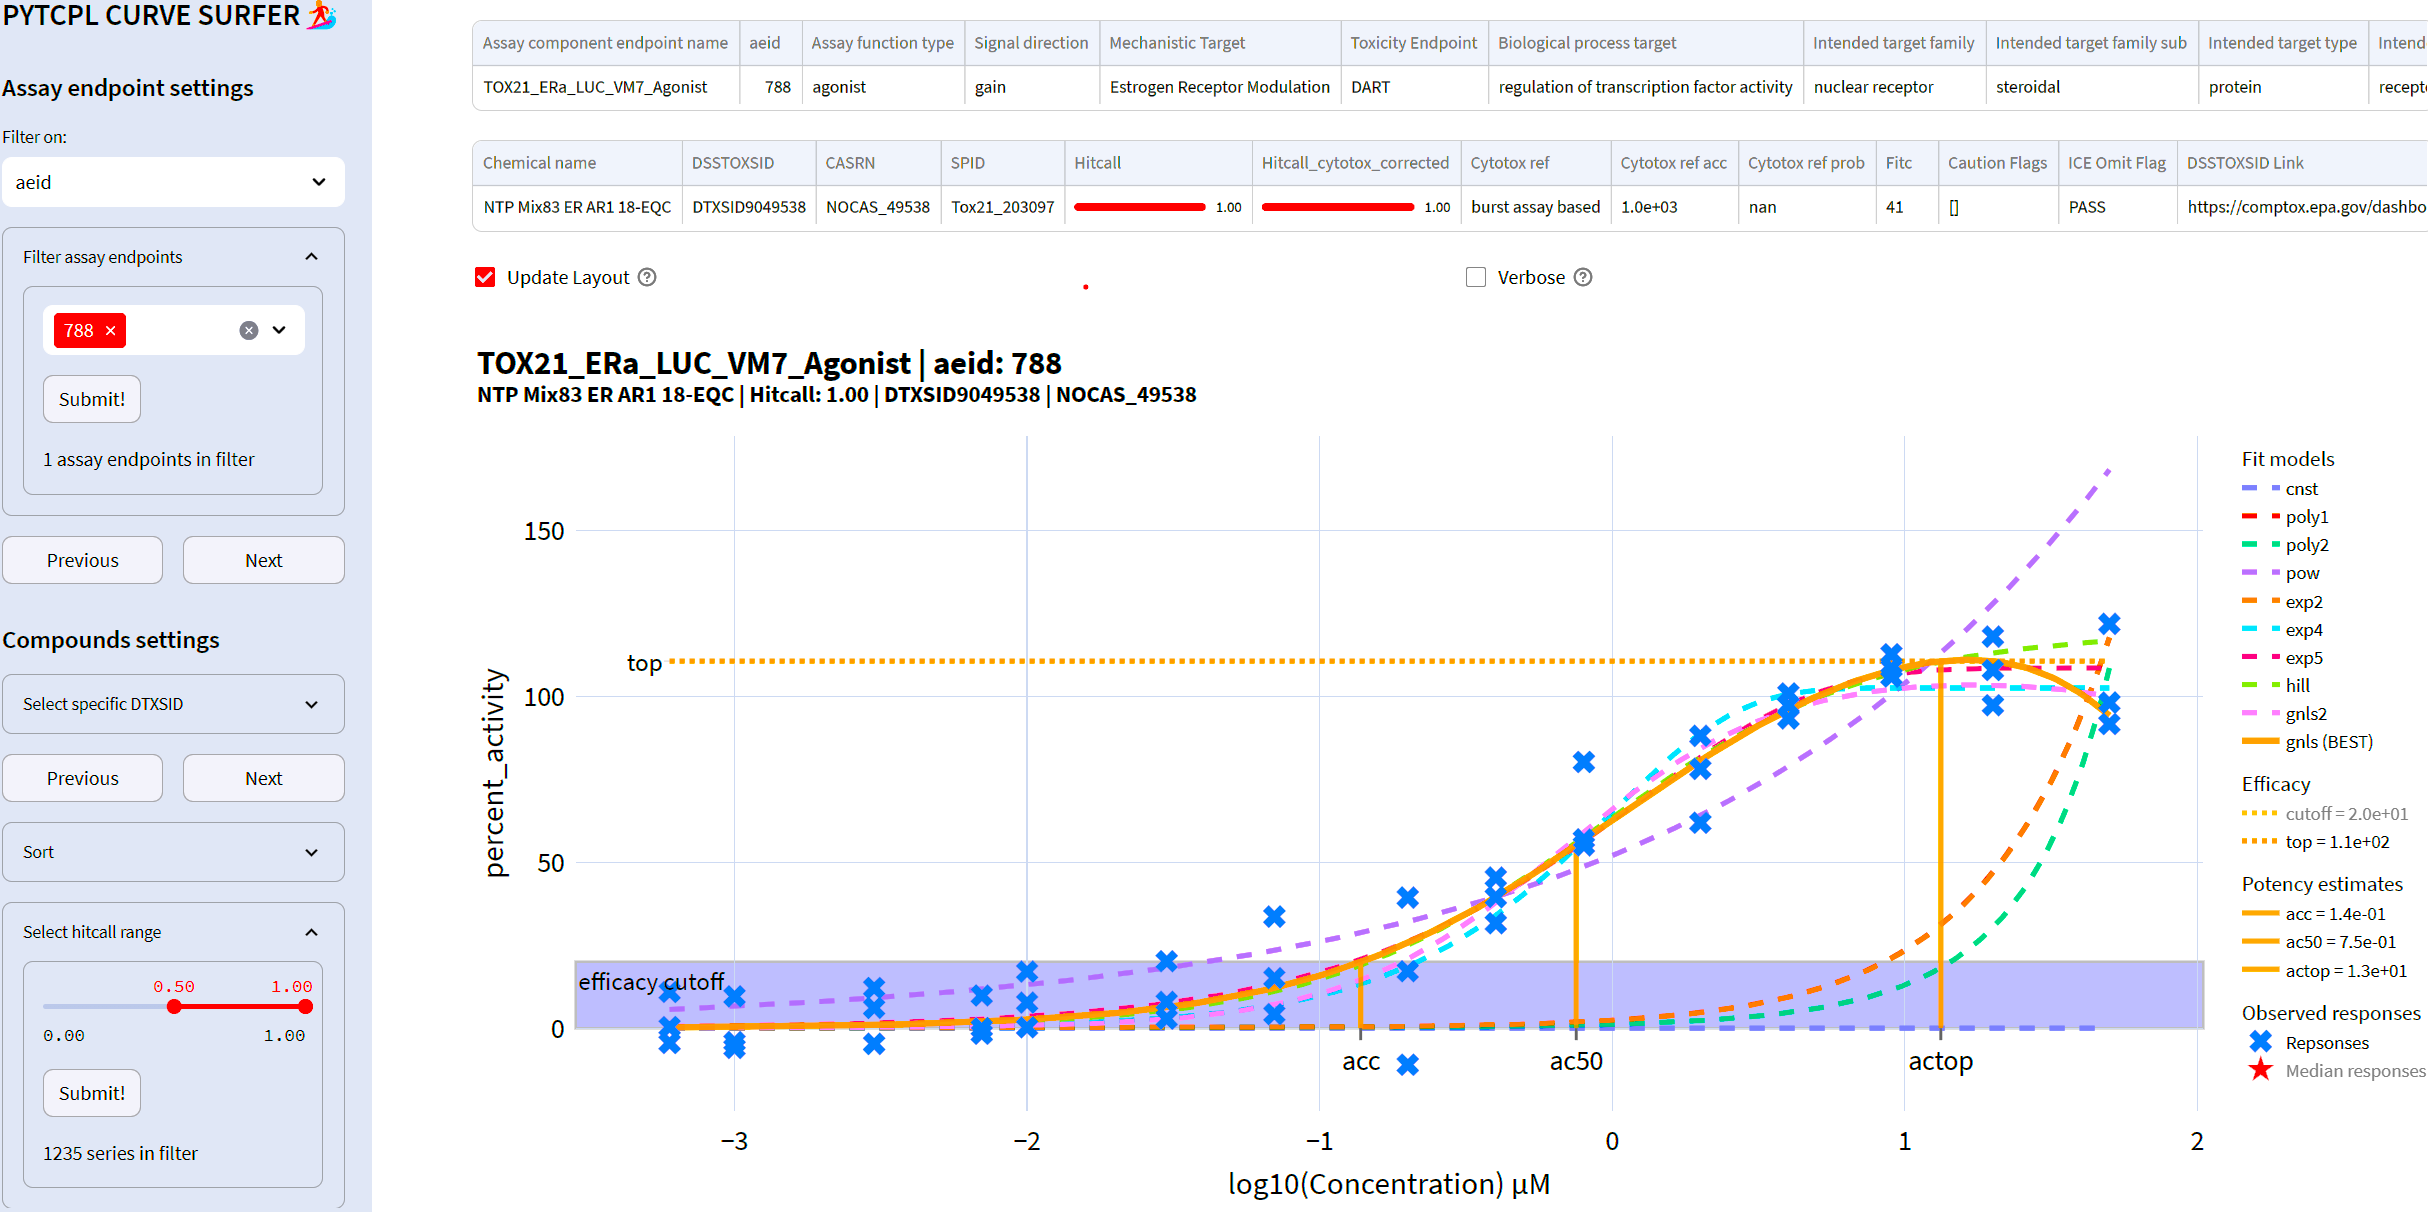
\includegraphics[width=1.0\textwidth]{figures/curve_surfer.png}
    \caption{The curve surfer provides the capability to narrow down assay endpoints based on critical annotations, and compounds can be selectively filtered using their DTXSID. Users can navigate through assay endpoints or the compounds within the current assay endpoint. Additionally, compounds can be filtered by their hitcall value or POD estimates using a range slider. Subsequently, the curve surfer displays comprehensive details for the chosen compound within the opted assay endpoint, showcasing CRS data along with curve fit models and metadata.}
~\label{fig:curve_surfer}
\end{figure}


\section{Toxicity Prediction from Molecular Fingerprints: Machine Learning Pipeline}
The primary goal is to develop individual machine learning models for each assay endpoint, enabling the prediction of assay-specific compound toxicity based on molecular structure inputs. These models utilize molecular fingerprints to predict compound toxicity, as illustrated in Figure~\ref{fig:ml_dataset}. Please take into consideration that we utilized both binary classification and regression models. In the case of binary classification, we applied a threshold of $0.5$ to convert the continuous hitcall target values into binary outcomes.

To create these individual datasets, we extract compounds that possess toxicity data for a given assay endpoint from the outputs generated by pytcpl. The associated hitcall values for these compounds are used as target variables within the machine learning model.

The binary input features for the model consist of molecular fingerprints derived from chemical structures. The structural data was obtained from the U.S. EPA's DSSTox database, accessed through the CompTox Chemicals Dashboard. The structural data mining and the necessary structure cleanup, as mentioned in Section~\ref{sec:toxicity_testing}, was conducted by Dr.\ Kasia Arturi\footnote{\url{https://gitlab.renkulab.io/expectmine/generating-fingerprints}}.

\begin{figure} 
    \centering
    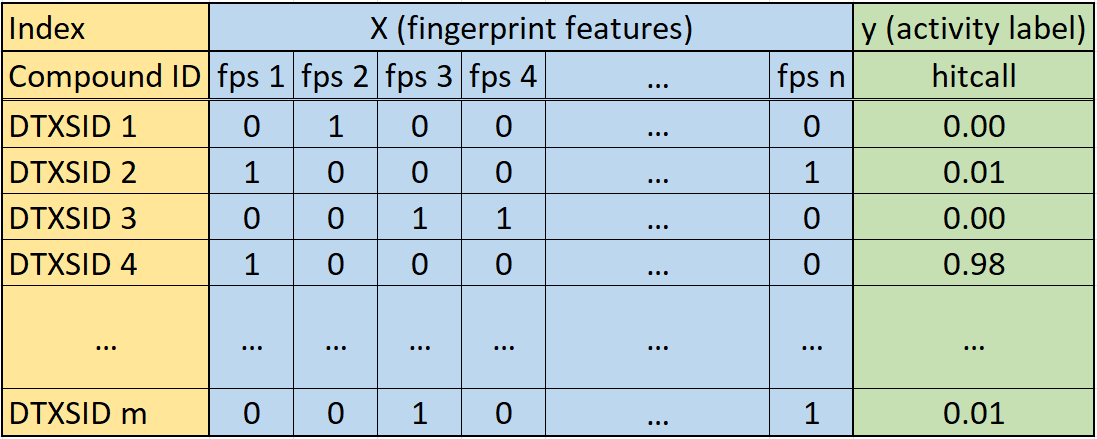
\includegraphics[width=0.8\textwidth]{figures/ml_dataset.png}
    \caption{Schematic example of a machine learning dataset related to a single assay endpoint. The dataset is structured into a feature matrix and a target vector. The feature matrix consists of molecular fingerprints, and the target vector is the hitcall value. For binary classification, the hitcall value is binarized based on a specific activity threshold.}
~\label{fig:ml_dataset}
\end{figure}


The machine learning pipeline is structured into three main stages: model training, model evaluation and model application. The following sections and the Figure illustrated in Figure~\ref{fig:Project_overview} provide a detailed description of each stage.

\begin{figure}
    \centering
    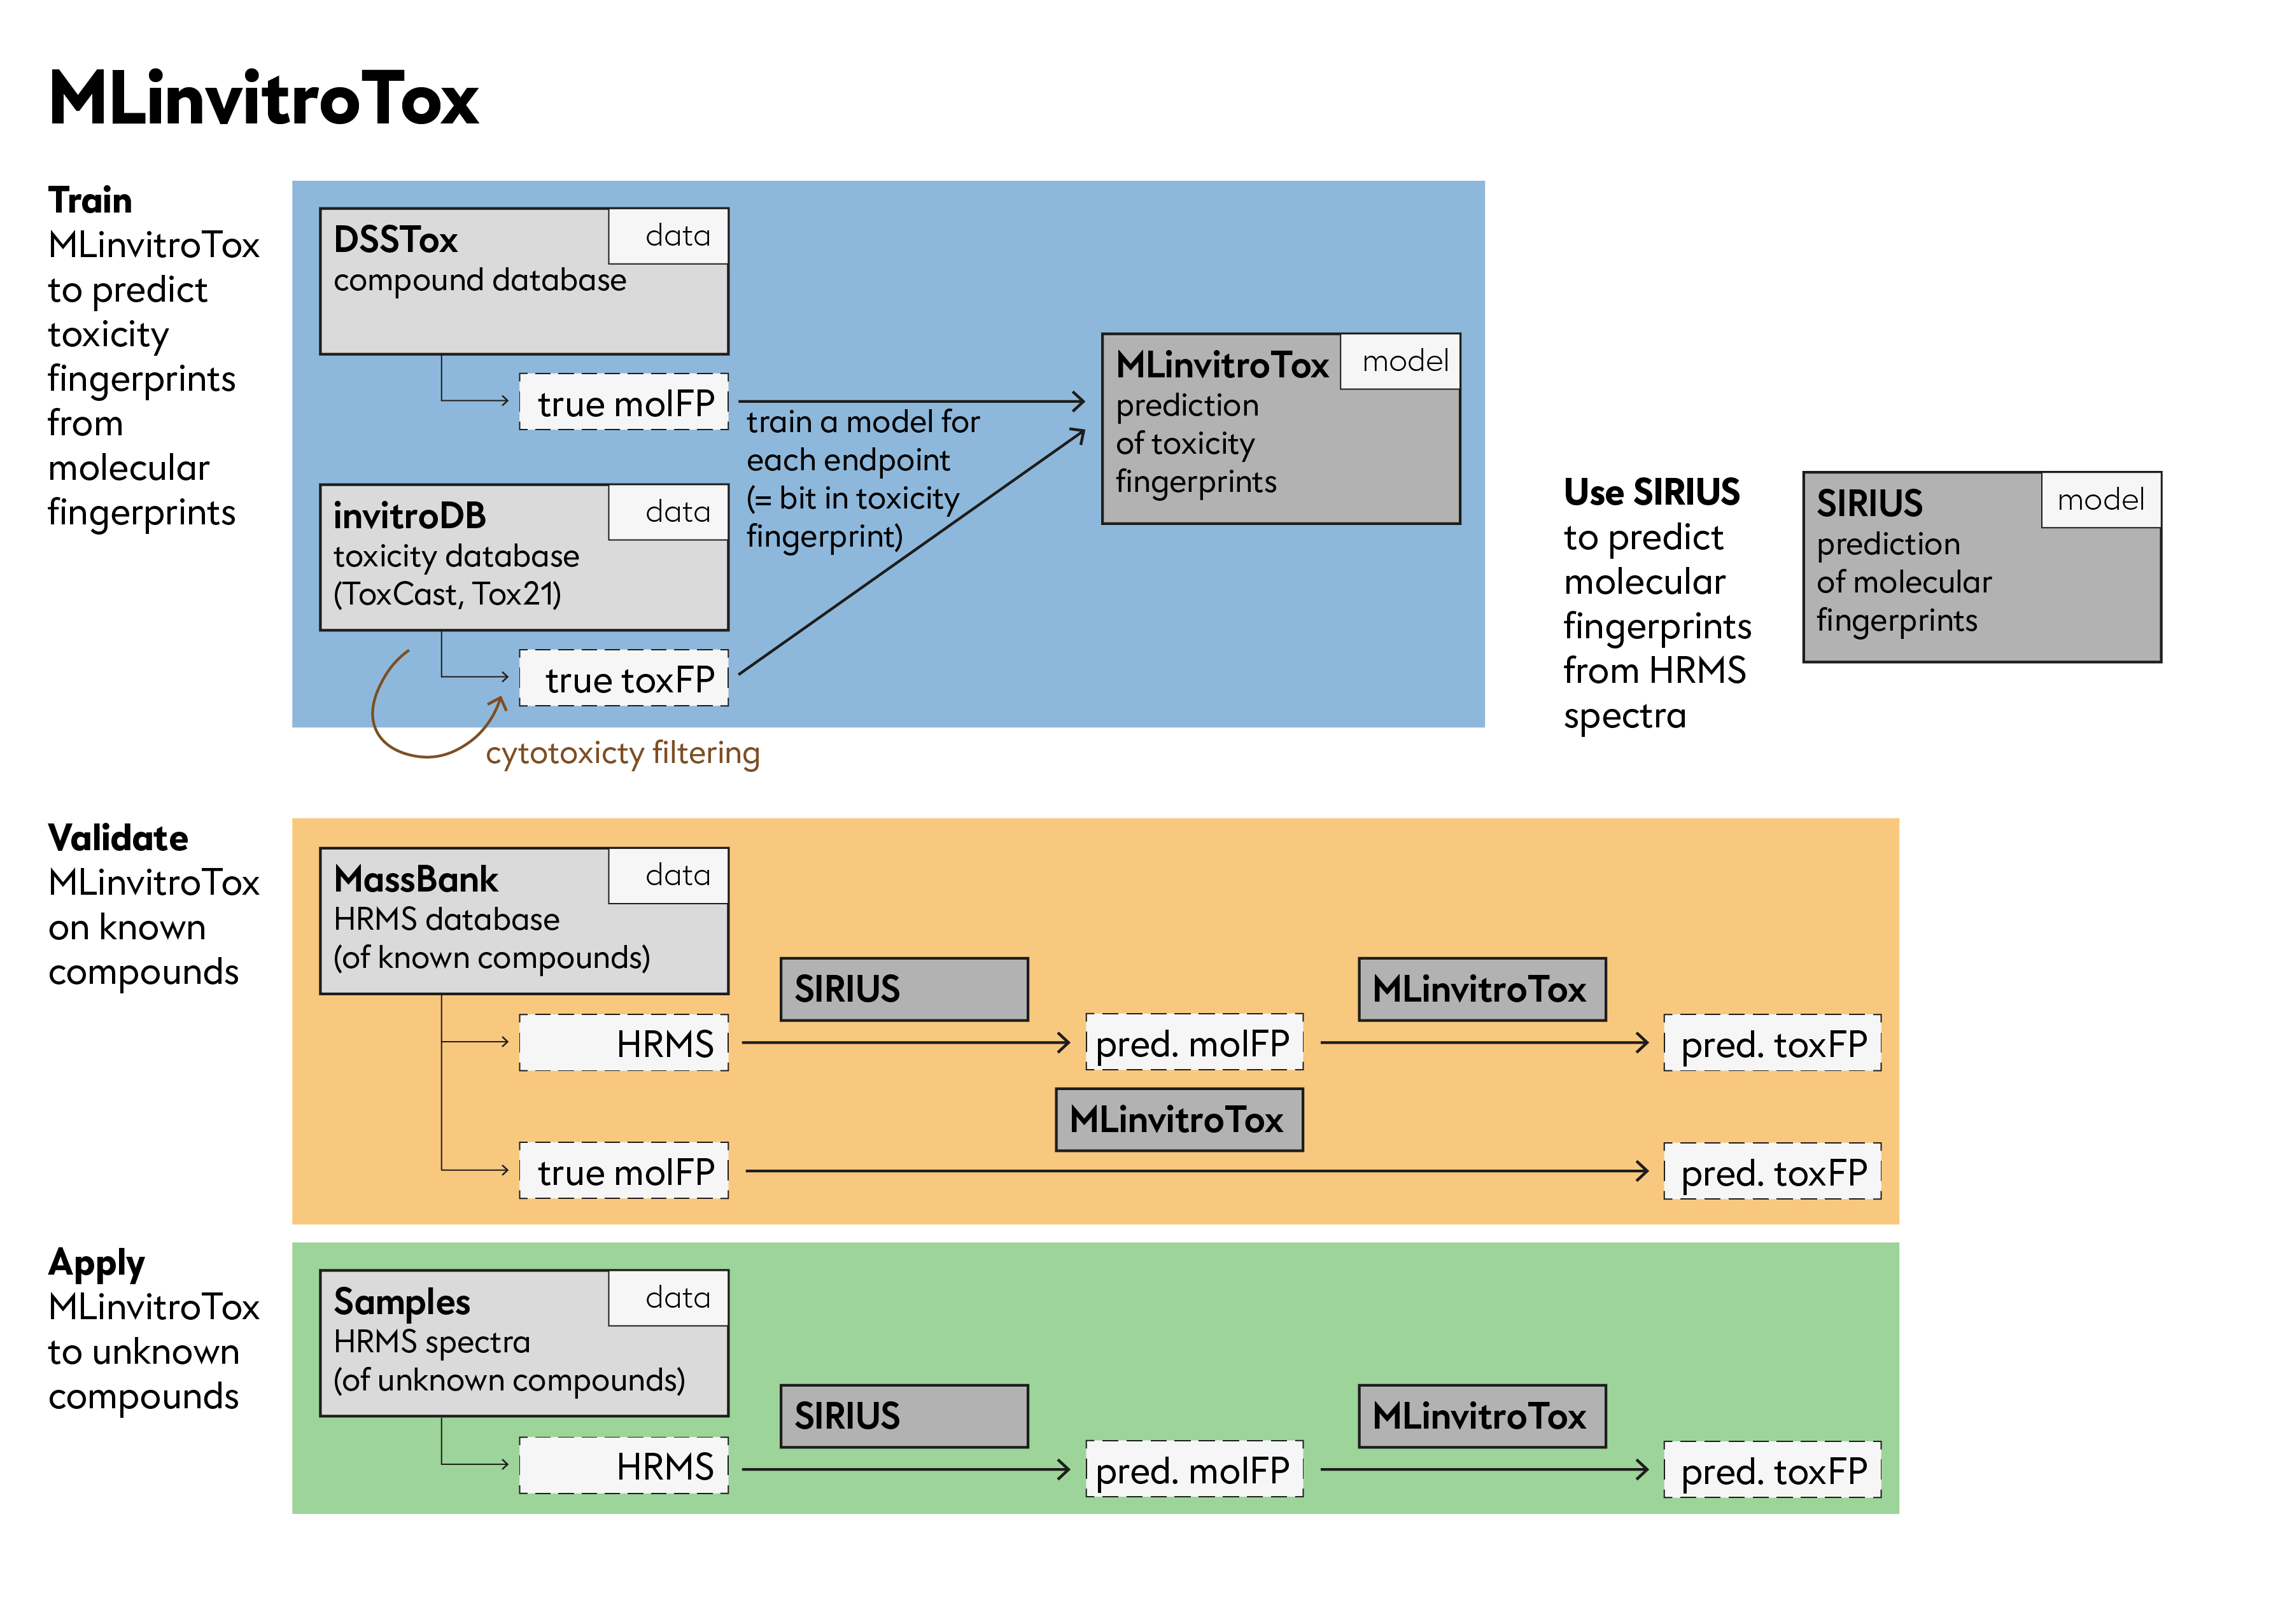
\includegraphics[width=1.0\textwidth]{figures/Project_overview.png}
    \caption{MLinvitroTox: Machine Learning Pipeline Steps. Figure created by Lili Gasser.}
~\label{fig:Project_overview}
\end{figure}

\subsection{Training}
The train stage is summarized in Figure~\ref{fig:Project_overview_train} and involves the generation of individual machine learning models for each assay endpoint. Each model is trained on a subset of the dataset with a 80/20 train/validation split. 

\begin{figure} 
    \centering
    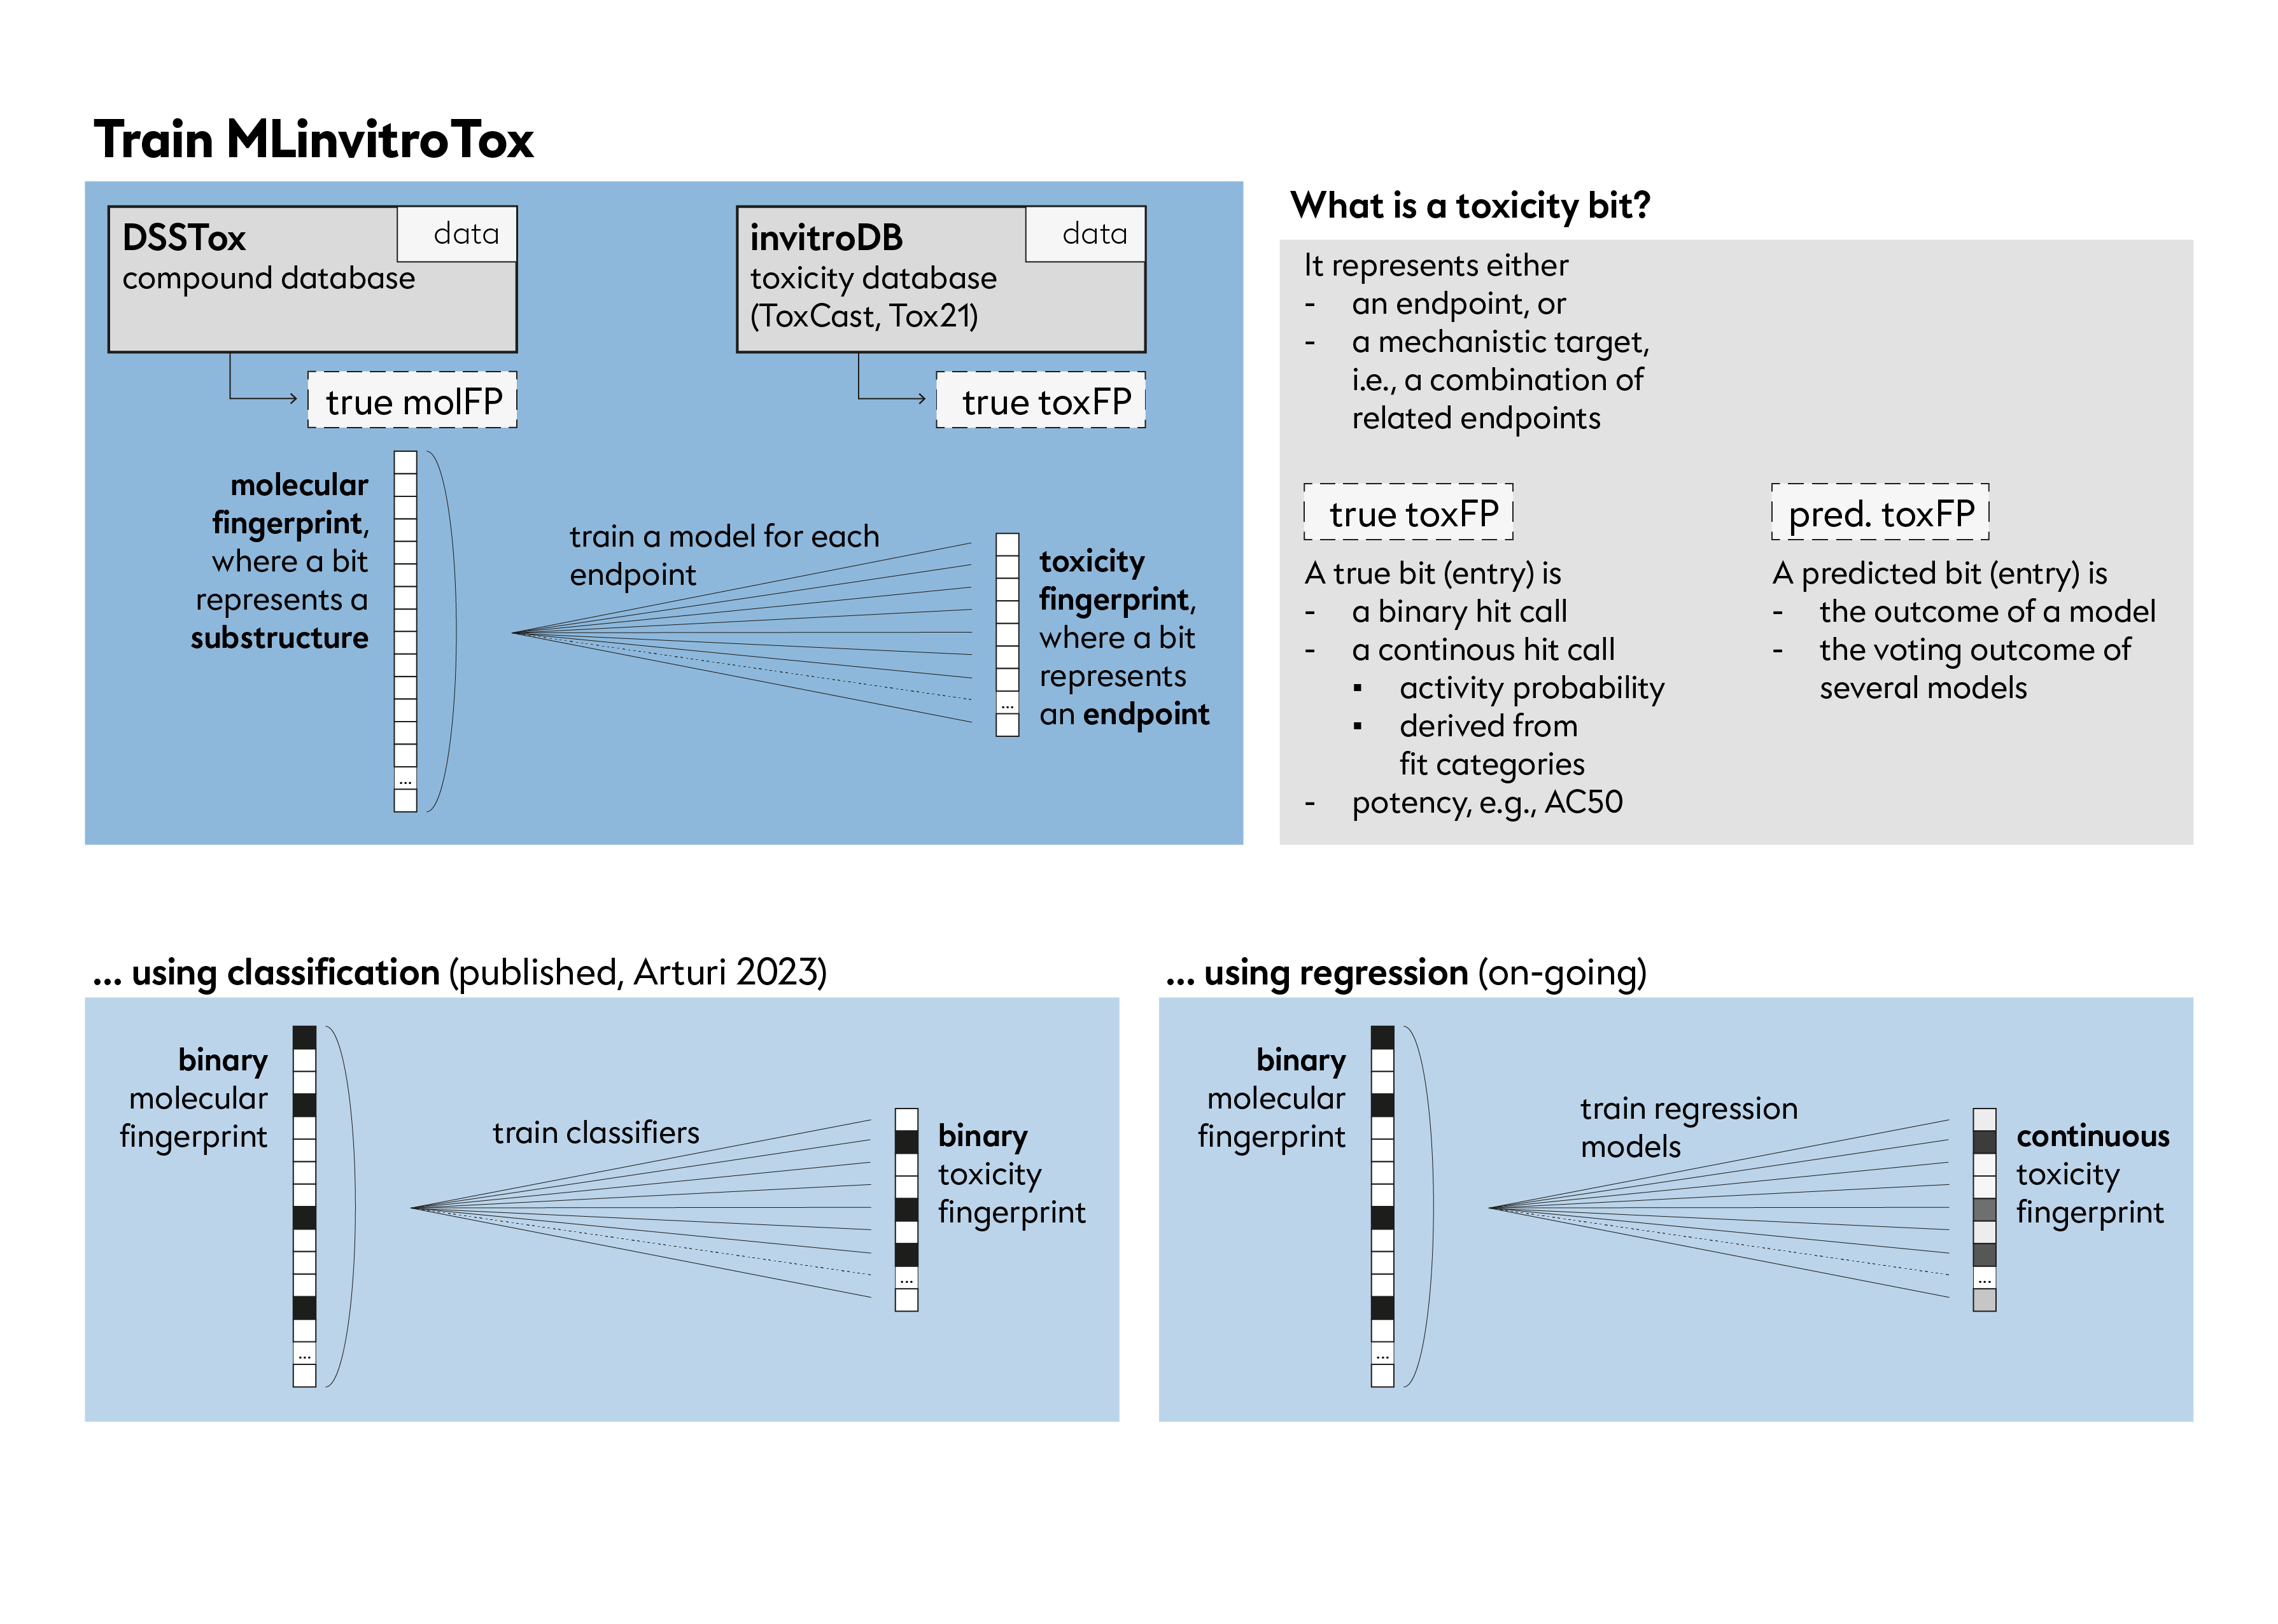
\includegraphics[width=1.0\textwidth]{figures/Project_overview_train.png}
    \caption{MLinvitroTox Train Step. Figure created by Lili Gasser.}
~\label{fig:Project_overview_train}
\end{figure}

\subsubsection{Feature Selection}
For all models we do feature selection based on machine learning model that extracts the most important features. This is then used as a transformer on the input data. The XGBoost model was used for this purpose. The number of features to be selected was determined by the number of features that reach the mean feature importance. 
\subsubsection{Model Selection}
The following supervised machine learning models from the \texttt{scikit-learn} library were considered for this thesis: 
\begin{enumerate}
    \item \textbf{Logistic Regression} is a linear model that utilizes the logistic function to model binary dependent variables. It serves as a straightforward and interpretable model, often employed as a baseline for binary classification tasks.
    \item \textbf{Support Vector Machine}: is a robust model with a lower susceptibility to overfitting and the ability to handle high-dimensional feature spaces.
    \item \textbf{Random Forest} is a bagging (bootstrap aggregating) ensemble learning technique in machine learning that constructs a multitude of decision trees during training and combines their predictions, resulting in robust and accurate models with the advantage of reduced overfitting and the ability to handle high-dimensional data.
    \item \textbf{XGBoost} is a gradient boosting ensemble learning technique that combines multiple weak learner decision trees sequentially, with each new learner giving more weight to the examples that the previous learners struggled with. It provides typically high predictive accuracy and efficiency through techniques like gradient optimization and regularization.
    \item \textbf{Multi-Layer Perceptron} is a type of artificial neural network that consists of multiple layers of interconnected neurons and is used for various machine learning tasks, offering the advantage of modeling complex non-linear relationships in data.
\end{enumerate}

For every machine learning model, the selection process is based on a grid search over a set of hyperparameters, using 5-fold cross-validation. The hyperparameters, specified in a seperate config file, are optimized for binary classification based on the $\text{F}_{\beta}$ score, a generalization of the $\text{F}_{1}$. The $\text{F}_{1}$-score is the harmonic mean of the precision and recall and the more generic $\text{F}_{\beta}$ score applies additional weights, valuing one of precision or recall more than the other. We set $\beta=2$ to value recall more than precision. 


\subsection{Evaluation}
To assess the performance of our trained models, we used two separate validation sets that were not part of the training data:


The first straightforward validation set, was utilized to evaluate how well the the best estimator found by the grid search 5-fold cross-validation generalizes for unseen compounds. This set was randomly sampled from the tested compounds in the specific assay endpoints, ensuring that the number of active and inactive compounds was balanced.

The MassBank validation set, serving as the second validation set, was utilized to evaluate the model's generalization capabilities, specifically examining the disparity between chemical structure space and fragmentation spectra. This evaluation is pivotal as it assesses the model's performance during its application stage. Prior to any further data splitting, this subset of compounds was separated. This subset includes compounds for which we have access to both actual and SIRIUS predicted fingerprints originating from MassBank spectra data. The availability of both sets of fingerprints enables us to assess the reliability of the predicted fingerprints as indicators of compound toxicity. This assessment is carried out by comparing the models' performance on both the actual and predicted fingerprints.   

It is worth noting that potentially data-leaking compounds were excluded that were used in training the SIRIUS+CSI:FingerID prediction model itself, leaving us with a maximum of 315 compounds that can be safely used for MassBank validation. However, the MassBank validation set's size varies for different assay endpoints due to differences in the overlap between the compounds tested in MassBank spectra data and those present in the toxicity data, despite the fixed number of compounds available in MassBank spectra data, illustrated in Figure~\ref{fig:Massbank_validation}. Moreover the the representativenes of the validation set is illustrated in Figure~\ref{fig:activity_ratio_comparison}.


\begin{figure}
    \centering
    \begin{subfigure}[b]{0.48\textwidth}
        \centering
        \includegraphics[width=\textwidth]{figures/Massbank_overlap.png}
        \caption{The Overlap between compounds for that we have MassBank spectra data and compounds we have toxicity data. The number of compounds in the MassBank validation set varies for different assay endpoints due to differences in the overlap between the compounds tested in MassBank spectra data and those present in the toxicity data.}
    ~\label{fig:MassBank_overlap}
    \end{subfigure}
    \hfill
    \begin{subfigure}[b]{0.48\textwidth}
        \centering
        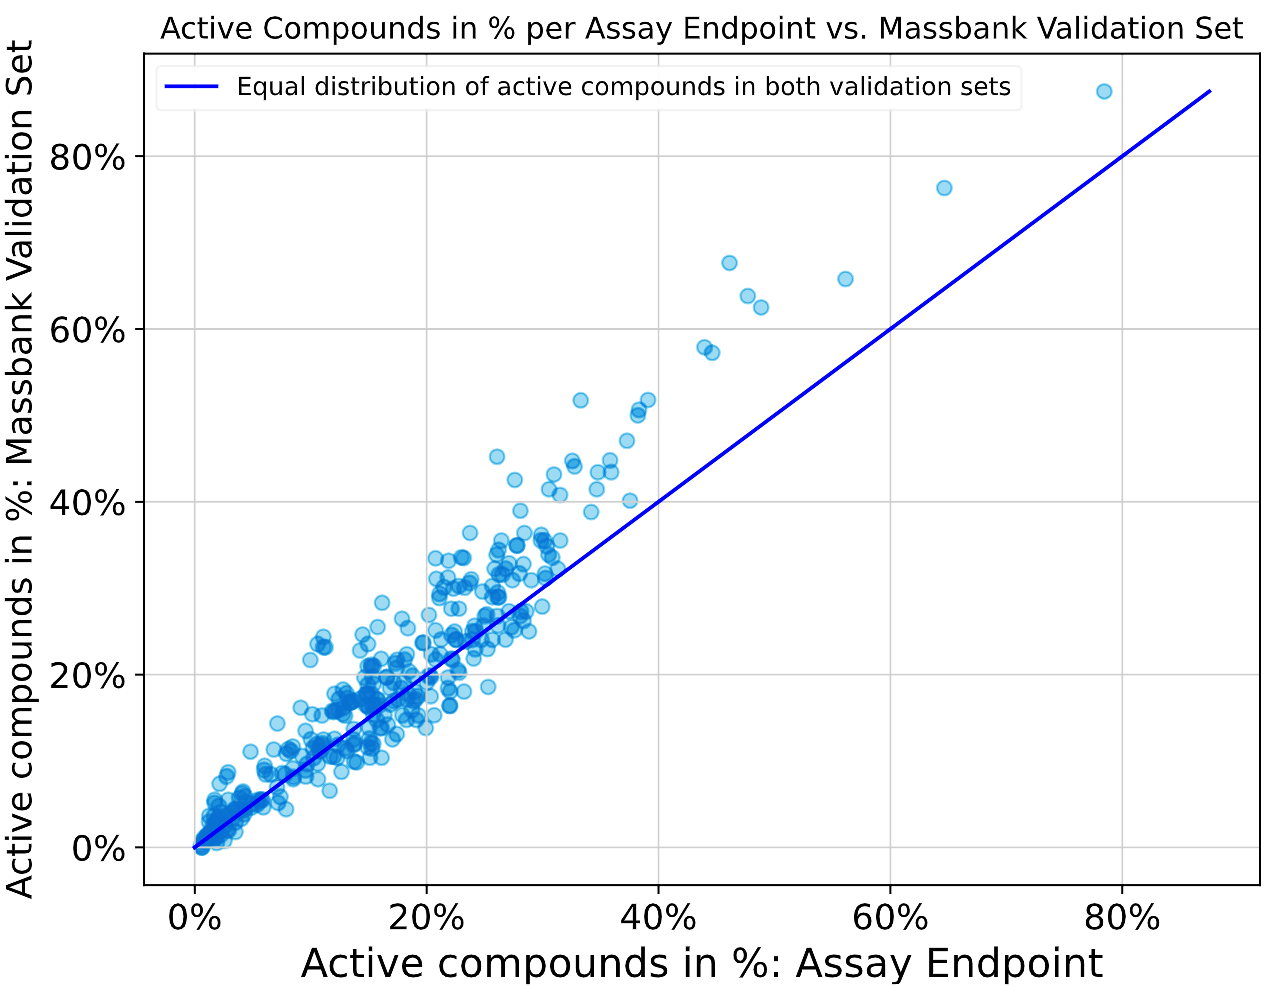
\includegraphics[width=\textwidth]{figures/activity_ratio_comparison.png}
        \caption{Plotting the ratio of active (binarized) hitcall values for all compounds tested in the assay endpoint against the ratio of active (binarized) hitcall values for the compounds in the MassBank validation set. The line represents the ideal case where the ratios are equal and the validation set is representative of the entire dataset.}
        ~\label{fig:activity_ratio_comparison}
    \end{subfigure}
    \caption{MassBank validation set.}
    ~\label{fig:Massbank_validation}
\end{figure}


\subsection{Application}
The presence of distinct prediction models for each assay endpoint enables the grouping of these endpoints based on their annotations, such as the biological process or the mechanistic target annotation. This ultimately results in toxicity predictions averaged within these groups. These collective toxicity predictions are referred to as \emph{toxicity fingerprint} which serve the purpose of identifying the most toxic compounds for each specific assay endpoint.


